%Manuscript based on tutorial given by Fred J. Hickernell at MCQMC, August 14, 2016
%Requires graphics files
% L2Kernel.eps, LocalDiscrep.eps, IIDPoints.eps, ShiftedLatticePoints.eps, 
% USobolPoints.eps, SSobolPoints.eps, UnwtL2Disclat.eps, UnwtL2Disc.eps, 
% MVNIIDUSobolSobol.eps, MVNSobolGenzAff, GenzFun.eps, AffineFun.eps,
% AsianCallIIDUSobolSobol.eps, AsianCallSobolPCADiff.eps, Matern.eps, 
% MVNIIDUSobolSobolWtSobol.eps, MVNSobolWtSobolErrBd.eps, WtL2Disclat.eps,   
% WtL2Disc.eps


\documentclass[graybox,footinfo]{svmult}

\smartqed
\usepackage{mathptmx}       % selects Times Roman as basic font
\usepackage{helvet}         % selects Helvetica as sans-serif font
\usepackage{courier}        % selects Courier as typewriter font
\usepackage{type1cm}        % activate if the above 3 fonts are
% not available on your system
\usepackage{graphicx}       % standard LaTeX graphics tool
% when including figure files

\usepackage{array,colortbl}
\usepackage{amsmath,amsfonts,amssymb,bm} % no amsthm, Springer defines Theorem, 
%Lemma, etc themselves
%\usepackage[mathx]{mathabx}
\DeclareFontFamily{U}{mathx}{\hyphenchar\font45}
\DeclareFontShape{U}{mathx}{m}{n}{
	<5> <6> <7> <8> <9> <10>
	<10.95> <12> <14.4> <17.28> <20.74> <24.88>
	mathx10
}{}
\DeclareSymbolFont{mathx}{U}{mathx}{m}{n}
\DeclareFontSubstitution{U}{mathx}{m}{n}
\DeclareMathAccent{\widecheck}      {0}{mathx}{"71}



% Note that Springer defines the following already:
%
% \D upright d for differential d
% \I upright i for imaginary unit
% \E upright e for exponential function
% \tens depicts tensors as sans serif upright
% \vec depicts vectors as boldface characters instead of the arrow accent
%
% Additionally we throw in the following common used macro's:
%%  This file will be included when we compile the final book. You can
%%  make use of the commonly used packages and commonly defined macros
%%  from here.
%%
%%  PLEASE DO NOT CHANGE THIS FILE.
%%  PLEASE DO NOT REDFINE ANY OF THE MACROS.
%%
%%  For convenience you may wish to define your own macros in your main
%%  tex file while preparing the manuscript. However, before submitting
%%  your final file for the accepted manuscript, we will ask you to replace
%%  your macros with the full commands.
%%

\renewcommand{\email}[1]{\emailname: #1} % change the email address font style

\usepackage{mathptmx}       % selects Times Roman as basic font
\usepackage{helvet}         % selects Helvetica as sans-serif font
\usepackage{courier}        % selects Courier as typewriter font
%\usepackage{type1cm}        % activate if the above 3 fonts are
%                            % not available on your system

\usepackage{makeidx}         % allows index generation
\usepackage{graphicx}        % standard LaTeX graphics tool
                             % when including figure files
%\usepackage{multicol}        % used for the two-column index
\usepackage[bottom]{footmisc}% places footnotes at page bottom

\usepackage{latexsym}
\usepackage{amsmath}
\usepackage{amsfonts}
\usepackage{amssymb}
\usepackage{bm}

\usepackage{url}
\usepackage{algorithm}
\usepackage{algorithmic}
\usepackage[misc,geometry]{ifsym}

% Springer provides the following environments:
%   case, conjecture, corollary, definition, example, exercise, lemma,
%   note, problem, property, proposition, question, remark, solution, theorem
%   claim, proof
\renewenvironment{proof}{\noindent{\itshape Proof.}}{\smartqed\qed}

% We add two more environments:   assumption, algo
\spdefaulttheorem{assumption}{Assumption}{\upshape \bfseries}{\itshape}
\spdefaulttheorem{algo}{Algorithm}{\upshape \bfseries}{\itshape}
% Note there is also the 'algorithm' environment from the algorithm package
% which is a floating environment



% Springer defines the following commands in math mode:
%   \D upright d for differential d
%   \I upright i for imaginary unit
%   \E upright e for exponential function
%   \tens depicts tensors as sans serif upright
%   \vec depicts vectors as boldface characters instead of the arrow accent


% We add the following commonly used macros:

% vectors as boldsymbols:
\newcommand{\bsa}{{\boldsymbol{a}}}
\newcommand{\bsb}{{\boldsymbol{b}}}
\newcommand{\bsc}{{\boldsymbol{c}}}
\newcommand{\bsd}{{\boldsymbol{d}}}
\newcommand{\bse}{{\boldsymbol{e}}}
\newcommand{\bsf}{{\boldsymbol{f}}}
\newcommand{\bsg}{{\boldsymbol{g}}}
\newcommand{\bsh}{{\boldsymbol{h}}}
\newcommand{\bsi}{{\boldsymbol{i}}}
\newcommand{\bsj}{{\boldsymbol{j}}}
\newcommand{\bsk}{{\boldsymbol{k}}}
\newcommand{\bsl}{{\boldsymbol{l}}}
\newcommand{\bsm}{{\boldsymbol{m}}}
\newcommand{\bsn}{{\boldsymbol{n}}}
\newcommand{\bso}{{\boldsymbol{o}}}
\newcommand{\bsp}{{\boldsymbol{p}}}
\newcommand{\bsq}{{\boldsymbol{q}}}
\newcommand{\bsr}{{\boldsymbol{r}}}
\newcommand{\bss}{{\boldsymbol{s}}}
\newcommand{\bst}{{\boldsymbol{t}}}
\newcommand{\bsu}{{\boldsymbol{u}}}
\newcommand{\bsv}{{\boldsymbol{v}}}
\newcommand{\bsw}{{\boldsymbol{w}}}
\newcommand{\bsx}{{\boldsymbol{x}}}
\newcommand{\bsy}{{\boldsymbol{y}}}
\newcommand{\bsz}{{\boldsymbol{z}}}
\newcommand{\bsA}{{\boldsymbol{A}}}
\newcommand{\bsB}{{\boldsymbol{B}}}
\newcommand{\bsC}{{\boldsymbol{C}}}
\newcommand{\bsD}{{\boldsymbol{D}}}
\newcommand{\bsE}{{\boldsymbol{E}}}
\newcommand{\bsF}{{\boldsymbol{F}}}
\newcommand{\bsG}{{\boldsymbol{G}}}
\newcommand{\bsH}{{\boldsymbol{H}}}
\newcommand{\bsI}{{\boldsymbol{I}}}
\newcommand{\bsJ}{{\boldsymbol{J}}}
\newcommand{\bsK}{{\boldsymbol{K}}}
\newcommand{\bsL}{{\boldsymbol{L}}}
\newcommand{\bsM}{{\boldsymbol{M}}}
\newcommand{\bsN}{{\boldsymbol{N}}}
\newcommand{\bsO}{{\boldsymbol{O}}}
\newcommand{\bsP}{{\boldsymbol{P}}}
\newcommand{\bsQ}{{\boldsymbol{Q}}}
\newcommand{\bsR}{{\boldsymbol{R}}}
\newcommand{\bsS}{{\boldsymbol{S}}}
\newcommand{\bsT}{{\boldsymbol{T}}}
\newcommand{\bsU}{{\boldsymbol{U}}}
\newcommand{\bsV}{{\boldsymbol{V}}}
\newcommand{\bsW}{{\boldsymbol{W}}}
\newcommand{\bsX}{{\boldsymbol{X}}}
\newcommand{\bsY}{{\boldsymbol{Y}}}
\newcommand{\bsZ}{{\boldsymbol{Z}}}
% other commonly used boldsymbols:
\newcommand{\bsell}{{\boldsymbol{\ell}}}
\newcommand{\bszero}{{\boldsymbol{0}}} % vector of zeros
\newcommand{\bsone}{{\boldsymbol{1}}}  % vector of ones
% boldsymbol greeks:
\newcommand{\bsalpha}{{\boldsymbol{\alpha}}}
\newcommand{\bsbeta}{{\boldsymbol{\beta}}}
\newcommand{\bsgamma}{{\boldsymbol{\gamma}}}
\newcommand{\bsdelta}{{\boldsymbol{\delta}}}
\newcommand{\bsepsilon}{{\boldsymbol{\epsilon}}}
\newcommand{\bsvarepsilon}{{\boldsymbol{\varepsilon}}}
\newcommand{\bszeta}{{\boldsymbol{\zeta}}}
\newcommand{\bseta}{{\boldsymbol{\eta}}}
\newcommand{\bstheta}{{\boldsymbol{\theta}}}
\newcommand{\bsvartheta}{{\boldsymbol{\vartheta}}}
\newcommand{\bskappa}{{\boldsymbol{\kappa}}}
\newcommand{\bslambda}{{\boldsymbol{\lambda}}}
\newcommand{\bsmu}{{\boldsymbol{\mu}}}
\newcommand{\bsnu}{{\boldsymbol{\nu}}}
\newcommand{\bsxi}{{\boldsymbol{\xi}}}
\newcommand{\bspi}{{\boldsymbol{\pi}}}
\newcommand{\bsvarpi}{{\boldsymbol{\varpi}}}
\newcommand{\bsrho}{{\boldsymbol{\rho}}}
\newcommand{\bsvarrho}{{\boldsymbol{\varrho}}}
\newcommand{\bssigma}{{\boldsymbol{\sigma}}}
\newcommand{\bsvarsigma}{{\boldsymbol{\varsigma}}}
\newcommand{\bstau}{{\boldsymbol{\tau}}}
\newcommand{\bsupsilon}{{\boldsymbol{\upsilon}}}
\newcommand{\bsphi}{{\boldsymbol{\phi}}}
\newcommand{\bsvarphi}{{\boldsymbol{\varphi}}}
\newcommand{\bschi}{{\boldsymbol{\chi}}}
\newcommand{\bspsi}{{\boldsymbol{\psi}}}
\newcommand{\bsomega}{{\boldsymbol{\omega}}}
\newcommand{\bsGamma}{{\boldsymbol{\Gamma}}}
\newcommand{\bsDelta}{{\boldsymbol{\Delta}}}
\newcommand{\bsTheta}{{\boldsymbol{\Theta}}}
\newcommand{\bsLambda}{{\boldsymbol{\Lambda}}}
\newcommand{\bsXi}{{\boldsymbol{\Xi}}}
\newcommand{\bsPi}{{\boldsymbol{\Pi}}}
\newcommand{\bsSigma}{{\boldsymbol{\Sigma}}}
\newcommand{\bsUpsilon}{{\boldsymbol{\Upsilon}}}
\newcommand{\bsPhi}{{\boldsymbol{\Phi}}}
\newcommand{\bsPsi}{{\boldsymbol{\Psi}}}
\newcommand{\bsOmega}{{\boldsymbol{\Omega}}}

% Roman fonts:
\newcommand{\rma}{{\mathrm{a}}}
\newcommand{\rmb}{{\mathrm{b}}}
\newcommand{\rmc}{{\mathrm{c}}}
\newcommand{\rmd}{{\mathrm{d}}}
\newcommand{\rme}{{\mathrm{e}}}
\newcommand{\rmf}{{\mathrm{f}}}
\newcommand{\rmg}{{\mathrm{g}}}
\newcommand{\rmh}{{\mathrm{h}}}
\newcommand{\rmi}{{\mathrm{i}}}
\newcommand{\rmj}{{\mathrm{j}}}
\newcommand{\rmk}{{\mathrm{k}}}
\newcommand{\rml}{{\mathrm{l}}}
\newcommand{\rmm}{{\mathrm{m}}}
\newcommand{\rmn}{{\mathrm{n}}}
\newcommand{\rmo}{{\mathrm{o}}}
\newcommand{\rmp}{{\mathrm{p}}}
\newcommand{\rmq}{{\mathrm{q}}}
\newcommand{\rmr}{{\mathrm{r}}}
\newcommand{\rms}{{\mathrm{s}}}
\newcommand{\rmt}{{\mathrm{t}}}
\newcommand{\rmu}{{\mathrm{u}}}
\newcommand{\rmv}{{\mathrm{v}}}
\newcommand{\rmw}{{\mathrm{w}}}
\newcommand{\rmx}{{\mathrm{x}}}
\newcommand{\rmy}{{\mathrm{y}}}
\newcommand{\rmz}{{\mathrm{z}}}
\newcommand{\rmA}{{\mathrm{A}}}
\newcommand{\rmB}{{\mathrm{B}}}
\newcommand{\rmC}{{\mathrm{C}}}
\newcommand{\rmD}{{\mathrm{D}}}
\newcommand{\rmE}{{\mathrm{E}}}
\newcommand{\rmF}{{\mathrm{F}}}
\newcommand{\rmG}{{\mathrm{G}}}
\newcommand{\rmH}{{\mathrm{H}}}
\newcommand{\rmI}{{\mathrm{I}}}
\newcommand{\rmJ}{{\mathrm{J}}}
\newcommand{\rmK}{{\mathrm{K}}}
\newcommand{\rmL}{{\mathrm{L}}}
\newcommand{\rmM}{{\mathrm{M}}}
\newcommand{\rmN}{{\mathrm{N}}}
\newcommand{\rmO}{{\mathrm{O}}}
\newcommand{\rmP}{{\mathrm{P}}}
\newcommand{\rmQ}{{\mathrm{Q}}}
\newcommand{\rmR}{{\mathrm{R}}}
\newcommand{\rmS}{{\mathrm{S}}}
\newcommand{\rmT}{{\mathrm{T}}}
\newcommand{\rmU}{{\mathrm{U}}}
\newcommand{\rmV}{{\mathrm{V}}}
\newcommand{\rmW}{{\mathrm{W}}}
\newcommand{\rmX}{{\mathrm{X}}}
\newcommand{\rmY}{{\mathrm{Y}}}
\newcommand{\rmZ}{{\mathrm{Z}}}
% also commonly defined
\newcommand{\rd}{{\mathrm{d}}}
\newcommand{\ri}{{\mathrm{i}}}

% blackboards:
\newcommand{\bbA}{{\mathbb{A}}}
\newcommand{\bbB}{{\mathbb{B}}}
\newcommand{\bbC}{{\mathbb{C}}}
\newcommand{\bbD}{{\mathbb{D}}}
\newcommand{\bbE}{{\mathbb{E}}}
\newcommand{\bbF}{{\mathbb{F}}}
\newcommand{\bbG}{{\mathbb{G}}}
\newcommand{\bbH}{{\mathbb{H}}}
\newcommand{\bbI}{{\mathbb{I}}}
\newcommand{\bbJ}{{\mathbb{J}}}
\newcommand{\bbK}{{\mathbb{K}}}
\newcommand{\bbL}{{\mathbb{L}}}
\newcommand{\bbM}{{\mathbb{M}}}
\newcommand{\bbN}{{\mathbb{N}}}
\newcommand{\bbO}{{\mathbb{O}}}
\newcommand{\bbP}{{\mathbb{P}}}
\newcommand{\bbQ}{{\mathbb{Q}}}
\newcommand{\bbR}{{\mathbb{R}}}
\newcommand{\bbS}{{\mathbb{S}}}
\newcommand{\bbT}{{\mathbb{T}}}
\newcommand{\bbU}{{\mathbb{U}}}
\newcommand{\bbV}{{\mathbb{V}}}
\newcommand{\bbW}{{\mathbb{W}}}
\newcommand{\bbX}{{\mathbb{X}}}
\newcommand{\bbY}{{\mathbb{Y}}}
\newcommand{\bbZ}{{\mathbb{Z}}}
% commonly used shortcuts:
\newcommand{\C}{{\mathbb{C}}} % complex numbers
\newcommand{\F}{{\mathbb{F}}} % field, finite field
\newcommand{\N}{{\mathbb{N}}} % natural numbers {1, 2, ...}
\newcommand{\Q}{{\mathbb{Q}}} % rationals
\newcommand{\R}{{\mathbb{R}}} % reals
\newcommand{\Z}{{\mathbb{Z}}} % integers
% more commonly used shortcuts:
\newcommand{\CC}{{\mathbb{C}}} % complex numbers
\newcommand{\FF}{{\mathbb{F}}} % field, finite field
\newcommand{\NN}{{\mathbb{N}}} % natural numbers {1, 2, ...}
\newcommand{\QQ}{{\mathbb{Q}}} % rationals
\newcommand{\RR}{{\mathbb{R}}} % reals
\newcommand{\ZZ}{{\mathbb{Z}}} % integers
% more commonly used shortcuts:
\newcommand{\EE}{{\mathbb{E}}}
\newcommand{\PP}{{\mathbb{P}}}
\newcommand{\TT}{{\mathbb{T}}}
\newcommand{\VV}{{\mathbb{V}}}
% and even more commonly used shortcuts:
\newcommand{\Complex}{{\mathbb{C}}}
\newcommand{\Integer}{{\mathbb{Z}}}
\newcommand{\Natural}{{\mathbb{N}}}
\newcommand{\Rational}{{\mathbb{Q}}}
\newcommand{\Real}{{\mathbb{R}}}
% indicator boldface 1:
\DeclareSymbolFont{bbold}{U}{bbold}{m}{n}
\DeclareSymbolFontAlphabet{\mathbbold}{bbold}
\newcommand{\ind}{{\mathbbold{1}}}
\newcommand{\bbone}{{\mathbbold{1}}}


% calligraphic letters:
\newcommand{\cala}{{\mathcal{a}}}
\newcommand{\calb}{{\mathcal{b}}}
\newcommand{\calc}{{\mathcal{c}}}
\newcommand{\cald}{{\mathcal{d}}}
\newcommand{\cale}{{\mathcal{e}}}
\newcommand{\calf}{{\mathcal{f}}}
\newcommand{\calg}{{\mathcal{g}}}
\newcommand{\calh}{{\mathcal{h}}}
\newcommand{\cali}{{\mathcal{i}}}
\newcommand{\calj}{{\mathcal{j}}}
\newcommand{\calk}{{\mathcal{k}}}
\newcommand{\call}{{\mathcal{l}}}
\newcommand{\calm}{{\mathcal{m}}}
\newcommand{\caln}{{\mathcal{n}}}
\newcommand{\calo}{{\mathcal{o}}}
\newcommand{\calp}{{\mathcal{p}}}
\newcommand{\calq}{{\mathcal{q}}}
\newcommand{\calr}{{\mathcal{r}}}
\newcommand{\cals}{{\mathcal{s}}}
\newcommand{\calt}{{\mathcal{t}}}
\newcommand{\calu}{{\mathcal{u}}}
\newcommand{\calv}{{\mathcal{v}}}
\newcommand{\calw}{{\mathcal{w}}}
\newcommand{\calx}{{\mathcal{x}}}
\newcommand{\caly}{{\mathcal{y}}}
\newcommand{\calz}{{\mathcal{z}}}
\newcommand{\calA}{{\mathcal{A}}}
\newcommand{\calB}{{\mathcal{B}}}
\newcommand{\calC}{{\mathcal{C}}}
\newcommand{\calD}{{\mathcal{D}}}
\newcommand{\calE}{{\mathcal{E}}}
\newcommand{\calF}{{\mathcal{F}}}
\newcommand{\calG}{{\mathcal{G}}}
\newcommand{\calH}{{\mathcal{H}}}
\newcommand{\calI}{{\mathcal{I}}}
\newcommand{\calJ}{{\mathcal{J}}}
\newcommand{\calK}{{\mathcal{K}}}
\newcommand{\calL}{{\mathcal{L}}}
\newcommand{\calM}{{\mathcal{M}}}
\newcommand{\calN}{{\mathcal{N}}}
\newcommand{\calO}{{\mathcal{O}}}
\newcommand{\calP}{{\mathcal{P}}}
\newcommand{\calQ}{{\mathcal{Q}}}
\newcommand{\calR}{{\mathcal{R}}}
\newcommand{\calS}{{\mathcal{S}}}
\newcommand{\calT}{{\mathcal{T}}}
\newcommand{\calU}{{\mathcal{U}}}
\newcommand{\calV}{{\mathcal{V}}}
\newcommand{\calW}{{\mathcal{W}}}
\newcommand{\calX}{{\mathcal{X}}}
\newcommand{\calY}{{\mathcal{Y}}}
\newcommand{\calZ}{{\mathcal{Z}}}

% Euler fraks:
\newcommand{\fraka}{{\mathfrak{a}}}
\newcommand{\frakb}{{\mathfrak{b}}}
\newcommand{\frakc}{{\mathfrak{c}}}
\newcommand{\frakd}{{\mathfrak{d}}}
\newcommand{\frake}{{\mathfrak{e}}}
\newcommand{\frakf}{{\mathfrak{f}}}
\newcommand{\frakg}{{\mathfrak{g}}}
\newcommand{\frakh}{{\mathfrak{h}}}
\newcommand{\fraki}{{\mathfrak{i}}}
\newcommand{\frakj}{{\mathfrak{j}}}
\newcommand{\frakk}{{\mathfrak{k}}}
\newcommand{\frakl}{{\mathfrak{l}}}
\newcommand{\frakm}{{\mathfrak{m}}}
\newcommand{\frakn}{{\mathfrak{n}}}
\newcommand{\frako}{{\mathfrak{o}}}
\newcommand{\frakp}{{\mathfrak{p}}}
\newcommand{\frakq}{{\mathfrak{q}}}
\newcommand{\frakr}{{\mathfrak{r}}}
\newcommand{\fraks}{{\mathfrak{s}}}
\newcommand{\frakt}{{\mathfrak{t}}}
\newcommand{\fraku}{{\mathfrak{u}}}
\newcommand{\frakv}{{\mathfrak{v}}}
\newcommand{\frakw}{{\mathfrak{w}}}
\newcommand{\frakx}{{\mathfrak{x}}}
\newcommand{\fraky}{{\mathfrak{y}}}
\newcommand{\frakz}{{\mathfrak{z}}}
\newcommand{\frakA}{{\mathfrak{A}}}
\newcommand{\frakB}{{\mathfrak{B}}}
\newcommand{\frakC}{{\mathfrak{C}}}
\newcommand{\frakD}{{\mathfrak{D}}}
\newcommand{\frakE}{{\mathfrak{E}}}
\newcommand{\frakF}{{\mathfrak{F}}}
\newcommand{\frakG}{{\mathfrak{G}}}
\newcommand{\frakH}{{\mathfrak{H}}}
\newcommand{\frakI}{{\mathfrak{I}}}
\newcommand{\frakJ}{{\mathfrak{J}}}
\newcommand{\frakK}{{\mathfrak{K}}}
\newcommand{\frakL}{{\mathfrak{L}}}
\newcommand{\frakM}{{\mathfrak{M}}}
\newcommand{\frakN}{{\mathfrak{N}}}
\newcommand{\frakO}{{\mathfrak{O}}}
\newcommand{\frakP}{{\mathfrak{P}}}
\newcommand{\frakQ}{{\mathfrak{Q}}}
\newcommand{\frakR}{{\mathfrak{R}}}
\newcommand{\frakS}{{\mathfrak{S}}}
\newcommand{\frakT}{{\mathfrak{T}}}
\newcommand{\frakU}{{\mathfrak{U}}}
\newcommand{\frakV}{{\mathfrak{V}}}
\newcommand{\frakW}{{\mathfrak{W}}}
\newcommand{\frakX}{{\mathfrak{X}}}
\newcommand{\frakY}{{\mathfrak{Y}}}
\newcommand{\frakZ}{{\mathfrak{Z}}}
% sets as Euler fraks:
\newcommand{\seta}{{\mathfrak{a}}}
\newcommand{\setb}{{\mathfrak{b}}}
\newcommand{\setc}{{\mathfrak{c}}}
\newcommand{\setd}{{\mathfrak{d}}}
\newcommand{\sete}{{\mathfrak{e}}}
\newcommand{\setf}{{\mathfrak{f}}}
\newcommand{\setg}{{\mathfrak{g}}}
\newcommand{\seth}{{\mathfrak{h}}}
\newcommand{\seti}{{\mathfrak{i}}}
\newcommand{\setj}{{\mathfrak{j}}}
\newcommand{\setk}{{\mathfrak{k}}}
\newcommand{\setl}{{\mathfrak{l}}}
\newcommand{\setm}{{\mathfrak{m}}}
\newcommand{\setn}{{\mathfrak{n}}}
\newcommand{\seto}{{\mathfrak{o}}}
\newcommand{\setp}{{\mathfrak{p}}}
\newcommand{\setq}{{\mathfrak{q}}}
\newcommand{\setr}{{\mathfrak{r}}}
\newcommand{\sets}{{\mathfrak{s}}}
\newcommand{\sett}{{\mathfrak{t}}}
\newcommand{\setu}{{\mathfrak{u}}}
\newcommand{\setv}{{\mathfrak{v}}}
\newcommand{\setw}{{\mathfrak{w}}}
\newcommand{\setx}{{\mathfrak{x}}}
\newcommand{\sety}{{\mathfrak{y}}}
\newcommand{\setz}{{\mathfrak{z}}}
\newcommand{\setA}{{\mathfrak{A}}}
\newcommand{\setB}{{\mathfrak{B}}}
\newcommand{\setC}{{\mathfrak{C}}}
\newcommand{\setD}{{\mathfrak{D}}}
\newcommand{\setE}{{\mathfrak{E}}}
\newcommand{\setF}{{\mathfrak{F}}}
\newcommand{\setG}{{\mathfrak{G}}}
\newcommand{\setH}{{\mathfrak{H}}}
\newcommand{\setI}{{\mathfrak{I}}}
\newcommand{\setJ}{{\mathfrak{J}}}
\newcommand{\setK}{{\mathfrak{K}}}
\newcommand{\setL}{{\mathfrak{L}}}
\newcommand{\setM}{{\mathfrak{M}}}
\newcommand{\setN}{{\mathfrak{N}}}
\newcommand{\setO}{{\mathfrak{O}}}
\newcommand{\setP}{{\mathfrak{P}}}
\newcommand{\setQ}{{\mathfrak{Q}}}
\newcommand{\setR}{{\mathfrak{R}}}
\newcommand{\setS}{{\mathfrak{S}}}
\newcommand{\setT}{{\mathfrak{T}}}
\newcommand{\setU}{{\mathfrak{U}}}
\newcommand{\setV}{{\mathfrak{V}}}
\newcommand{\setW}{{\mathfrak{W}}}
\newcommand{\setX}{{\mathfrak{X}}}
\newcommand{\setY}{{\mathfrak{Y}}}
\newcommand{\setZ}{{\mathfrak{Z}}}

% other commonly defined commands:
\newcommand{\wal}{{\rm wal}}
\newcommand{\floor}[1]{\left\lfloor #1 \right\rfloor} % floor
\newcommand{\ceil}[1]{\left\lceil #1 \right\rceil}    % ceil
\DeclareMathOperator{\cov}{Cov}
\DeclareMathOperator{\var}{Var}
\providecommand{\argmin}{\operatorname*{argmin}}
\providecommand{\argmax}{\operatorname*{argmax}}


% Macros below are now included in macros.tex from MCQMC 2016 web site
% This spot formerly included macros that are now in macros.tex

% indicator boldface 1:
\DeclareSymbolFont{bbold}{U}{bbold}{m}{n}
\DeclareSymbolFontAlphabet{\mathbbold}{bbold}
%\newcommand{\ind}{\mathbbold{1}}


\usepackage{microtype} % good font tricks

\usepackage[colorlinks=true,linkcolor=black,citecolor=black,urlcolor=black]{hyperref}
\urlstyle{same}
\usepackage{bookmark}
\pdfstringdefDisableCommands{\def\and{, }}
\makeatletter % to avoid hyperref warnings:
\providecommand*{\toclevel@author}{999}
\providecommand*{\toclevel@title}{0}
\makeatother

%%%%%%%%%%%%%%%%%%%%%%%%%%%%%%%%%%%%%%%%%%%%%%%%%%%%%%%%%%%%%%%%%%%%%%%%%%%%%%%%%%%%%%%%%


%Fred's additions
%
\usepackage{xspace}


%%%%%%%%%%%%%%%%%%%%%%%%%%%%%%%%%%%%%%%%%%%%%%%%%%%%%%%%%%%%%%%%%%%%%%%%%%%%%%%%%%%%%%%%%
\begin{document}
	
\newcommand{\FJHLessonZero}{The trio identity decomposes the cubature error as a 
	product of three factors: the variation of the integrand, the discrepancy of the 
	sampling measure, and the confounding. This identity shows how the integrand and 
	the sampling measure each contribute to the cubature error.  }	

\newcommand{\FJHLessonSix}{The trio identity has four versions, depending on whether 
the integrand is deterministic or Bayesian and whether the sampling measure is 
deterministic or random.  }

\newcommand{\FJHLessonTwoHalf}{The deterministic discrepancy when $\calF$ is an 
RKHS  has a simple, explicit form involving three factors. }	

\newcommand{\FJHLessonFourteen}{The formula for the Bayesian discrepancy mimics 
that for the deterministic discrepancy when $\calF$ is an RKHS. }	

\newcommand{\FJHLessonSeven}{Although it has traditionally been ignored, the 
confounding helps explain why the cubature error may decay to zero 
much faster or more slowly than the discrepancy.  }

\newcommand{\FJHLessonNine}{Bayesian cubature has a purely deterministic 
alternative interpretation.  }


	
\newcommand{\FJHQOne}{How do good sampling measures, $\hnu$, make 
the error smaller?}

\newcommand{\FJHLessonOne}{The quality of a sampling measure is important, not 
	merely the sample size.  Systematic sampling, even simple random sampling, may yield 
	a	much smaller error than haphazard sampling. }	

\newcommand{\FJHLessonTwo}{Quasi-Monte Carlo methods replace IID data sites by 
	low discrepancy data sites, such as
	Sobol' sequences and integration lattice nodeset sequences.  The resulting sampling 
	measures have discrepancies and cubature errors that decay to zero at 
	a faster rate than in the case of IID sampling. }


\newcommand{\FJHLessonThree}{Randomizing your sampling measure may not only 
	eliminate bias, but it may help you improve accuracy by avoiding the awful minority of 
	possible sampling measures. }

\newcommand{\FJHLessonFive}{The benefits of sampling measures with lower 
	discrepancy are limited to those problems where the integrand is well-behaved enough 
	to have finite variation.}





\newcommand{\FJHQTwo}{How can the error be decreased by re-casting the problem with a 
different integrand, $f$?}

\newcommand{\FJHLessonFour}{Well-chosen variable transformations may reduce 
	cubature error by producing an integrand with a smaller variation than the original. }

\newcommand{\FJHLessonEight}{The cubature error for high dimensional problems can often 
be reduced by arranging for 
the integrand to depend mainly on only several of the coordinates.  Moreover, those should 
preferably be the lower indexed coordinates. }

\newcommand{\FJHLessonTwelve}{Common variance reduction techniques used for IID 
Monte Carlo may also be applied for low discrepancy sampling measures. }

\newcommand{\FJHLessonThirteen}{Infinite dimensional problems may be efficiently solved 
by 
multi-level methods or multivariate decomposition methods, which approximate the integral 
by a sum of finite dimensional integrals. }




\newcommand{\FJHQThree}{How many samples, $n$, are required to meet a specified 
error tolerance?}

\newcommand{\FJHLessonTen}{Bayesian cubature, which assumes the integrand to be a 
Gaussian process, provides data-based probabilistic error bounds. }

\newcommand{\FJHLessonEleven}{Automatic stopping criteria for (quasi-) Monte Carlo 
simulations have been developed for integrands that are not too wild. }


\newcommand{\Cov}{\textup{cov}}
\newcommand{\algn}{\textup{CNF}}
\newcommand{\disc}{\textup{DSC}}
\newcommand{\Var}{\textup{VAR}}
%\DeclareMathOperator{\sign}{sign}
\newcommand{\GP}{\calG\!\!\calP}


\newlength{\FJHfigheight}
\setlength{\FJHfigheight}{4 cm}
	
\newtheorem{FJHLesson}{Lesson}
\newcommand{\corr}{\textup{corr}}
\newcommand{\std}{\textup{std}}
\newcommand{\Dt}{\textup{D}}
\newcommand{\Rn}{\textup{R}}
\newcommand{\Ba}{\textup{B}}
\newcommand{\tbsk}{\tilde{\bsk}}
\newcommand{\filC}{\widehat{C}}
\newcommand{\filc}{\widehat{c}}
\newcommand{\filbsc}{\widehat{\bsc}}
\newcommand{\filmC}{\widehat{\mathsf{C}}}

\newcommand{\MLE}{\text{MLE}}
\newcommand{\mC}{\mathsf{C}}
\newcommand{\tf}{\tilde{f}}
\newcommand{\hmu}{\widehat{\mu}}
\newcommand{\hnu}{\widehat{\nu}}
\newcommand{\norm}[1]{\ensuremath{\left \lVert #1 \right \rVert}} 
\newcommand{\snorm}[1]{\ensuremath{\left \lVert #1 \right \rVert}} 
\newcommand{\bignorm}[1]{\ensuremath{\bigl \lVert #1 \bigr \rVert}}
\newcommand{\Bignorm}[1]{\ensuremath{\Bigl \lVert #1 \Bigr \rVert}}
\newcommand{\abs}[1]{\ensuremath{\bigl \lvert #1 \bigr \rvert}}
\newcommand{\biggabs}[1]{\ensuremath{\biggl \lvert #1 \biggr \rvert}}
\newcommand{\ip}[3][{}]{\ensuremath{\left \langle #2, #3 \right \rangle_{#1}}}
\newcommand{\err}{\textrm{err}}
\newcommand{\tc}{\tilde{c}}
\newcommand{\tbsc}{\tilde{\bsc}}
\newcommand{\tmC}{\widetilde{\mC}}

\allowdisplaybreaks


\title*{Error Analysis for Quasi-Monte Carlo Methods}
\author{Fred J. Hickernell}
\institute{Fred J. Hickernell
\at Department of Applied Mathematics,  Illinois Institute of Technology, 10 W. 32$^{\text{nd}}$ Street, RE 208, Chicago, IL 60616, USA 
\email{hickernell@iit.edu}}
\maketitle

\abstract{Monte Carlo methods approximate integrals by sample averages 
of integrand values.  
The error of Monte Carlo methods may be expressed as a trio identity comprised of the 
variation of the integrand, the 
discrepancy of the sampling measure, and the 
confounding.  The trio identity has different versions, 
depending 
on whether  the integrand is deterministic or Bayesian and whether the sampling 
measure is 
deterministic or random.  Whereas the variation and the discrepancy are common in the 
literature, the confounding is a factor deserving more attention.   Theory 
and examples are used to show how the cuabature 
error may be reduced by employing the low discrepancy sampling that defines 
quasi-Monte Carlo 
methods.  The error may also be reduced  by rewriting the integral in terms of a different 
integrand.  Finally, the confounding  explains why the cubature error might not decay at a 
rate that one would expect from looking at the discrepancy.} 

\section{Introduction}
Monte Carlo methods are used to approximate multivariate integrals that cannot be evaluated analytically, i.e.,  integrals of the form
\begin{equation}
\mu = \int_{\calX} f(\bsx) \, \nu(\D \bsx), \label{FJH:eq:INT} \tag{INT}
\end{equation}
where $f:\calX \to \R$ is a measurable function, $\calX$ is a measurable set, and $\nu$ 
is a 
\emph{probability} measure.  Here, $\mu$ is the weighted average of the integrand, and 
it is also 
$\bbE[f(\bsX)]$, where the random variable $\bsX$ has probability measure $\nu$.  
Monte 
Carlo methods take the form of a weighted average of values of $f$ at a finite number of data 
sites, $\bsx_1, \ldots, \bsx_n$:
\begin{equation} \label{FJH:eq:AppxINT} \tag{MC}
\hmu = \sum_{i=1}^n f(\bsx_i) w_i = \int_{\calX} f(\bsx) \, \hnu(\D \bsx).
\end{equation}
The sampling measure, $\hnu$, assigns a weight $w_i$ to the function value at the 
$i^{\text{th}}$ data site, and lies in the vector space
\begin{equation} \label{FJH:eq:sampmeaset}
\calM_{\textup{S}} := \left \{\sum_{i=1}^n w_i \delta_{\bsx_i} : w_1, \ldots, w_n \in \R,\ 
\bsx_1, 
\ldots, \bsx_n \in \calX, \ n \in \N \right \},
\end{equation}
where  $\delta_{\bst}$ denotes a Dirac measure concentrated at point $\bst$. 

The data sites, the 
weights, and the sample size may be deterministic or random.  Later, we impose some 
constraints to facilitate 
the analysis.  We are 
particularly interested in sampling measures that choose the data sites more cleverly 
than independently and identically distributed (IID).  Such sampling measures are the 
hallmark of quasi-Monte Carlo methods.

This tutorial describes how to characterize and analyze the \emph{cubature error}, $\mu 
- \hmu$.  
Specifically, we ask
\begin{list}{}{\setlength\leftmargin{7ex}\setlength\labelwidth{5ex}}
\item[\emph{Question 1.}] \emph{\FJHQOne}
\item[\emph{Question 2.}] \emph{\FJHQTwo}
\item[\emph{Question 3.}] \emph{\FJHQThree}
\end{list}
\noindent We intersperse sixteen key lessons throughout this 
article and repeat them at the end.

\section{Big Data Survey} \label{FJH:sec:sleep} 
Did you get enough sleep last night?  Did you get more sleep than the average person?  
How much sleep did the average person get? The answer to this last question involves a 
simple sum:  $\mu = N^{-1} \sum_{j=1}^N f(j)$, where $f(j)$ 
denotes the hours of sleep of 
individual 
$j$ in a population of $N$ individuals.  For a large population, such as the $\approx 250$ 
million adults in the United States, an exhaustive sample is difficult to obtain. So you 
might resort to a 
web survey, where individuals $x_1, \ldots, x_n$ respond.  The error of 
your sample mean, $\widehat{\mu} = n^{-1} \sum_{i=1}^n f(x_i)$, may be decomposed as 
a 
product of three quantities:
\begin{align}
\nonumber
\mu - \widehat{\mu} 
&= \frac{1}N \sum_{j=1}^N f(j) -  \frac 1n \sum_{i=1}^n f(x_i)  = - \frac{1}N \sum_{j=1}^N \bigl[ f(j) 
- \mu \bigr]\left ( \frac Nn \bbone_{\{x_i\}_{i=1}^n}(j) 
- 1 \right) \\
& = \underbrace{-\corr(f, \bbone_{\{x_i\}_{i=1}^n})}_{\algn^\Dt(f,\nu - \hnu)} \,
\underbrace{\sqrt{\frac{1 - n/N}{n/N}}}_{\disc^\Dt(\nu - \hnu)} \, 
\underbrace{\std(f)}_{\Var^\Dt(f)}.
\label{FJH:eq:surveydettrio}
\end{align}
Here, the population covariance of two functions $f$ and $g$, with respective 
population means $\mu(f)$ and $\mu(g)$, is defined as 
\begin{equation*}
\Cov(f,g) : = \frac 1N \sum_{j=1} [f(j) - \mu(f)] [g(j) - \mu(g)], \qquad 
\std(f) : = \sqrt{\Cov(f,f)},
\end{equation*}
and direct calculation yields $\std\bigl((N/n)\bbone_{\{x_i\}_{i=1}^n}\bigr) = 
\sqrt{(1 - n/N)/(n/N)}$.

The expression of the error as a product of three factors in 
\eqref{FJH:eq:surveydettrio} is a case of the \emph{trio identity}, introduced by Meng 
\cite{Men16a}.  In this example the integral, $\mu$, corresponds to a sum, 
and the probability measure $\nu$ is the uniform measure over $\{1, 
\ldots, N\}$.  The sampling measure corresponding to the web survey is $\hnu = 
n^{-1} \sum_{i=1}^n \delta_{x_i}$.  The three factors that comprise the trio identity have 
the 
following meanings:
\begin{description}
	\item[$\Var(f)$] measures the \emph{variation} of the integrand from a typical value. 
	In 	this case, $\Var(f)$ corresponds to the standard deviation of $f$ and the typical 
	value	is the mean of $f$. The variation is positively homogeneous, i.e., $\Var(cf)  = 
	\abs{c} \Var(f)$.  The variation is \emph{not} the variance.
	\item [$\disc(\nu - \hnu)$] measures the \emph{discrepancy} of the sampling 
	measure 
	from the probability measure that defines the integral.  In this case, the discrepancy 
	depends only on the sample fraction, $n/N$, but in other cases it depends also on the 
	locations of the data sites.
	\item [$\algn(f,\nu - \hnu)$] measures the \emph{confounding} between the 
	integrand and the difference between the measure defining the integral and the 
	sampling measure.  In this case the confounding lies between plus and minus one.
\end{description}
The superscript $\Dt$ in \eqref{FJH:eq:surveydettrio} denotes a \emph{deterministic} 
version of the trio identity, which is defined in general in Sec.\ \ref{FJH:sec:dettrio}. 
Other versions of the trio identity are introduced later.

\begin{FJHLesson}
	\FJHLessonZero
\end{FJHLesson}

For the web survey example one might expect $\Var^\Dt(f)$ to be one or two hours.  It 
is an inherent quality of what we are measuring and is not affected by our sampling 
measure.  The discrepancy in this example will be quite large unless our survey includes a 
significant proportion of the population.  One might hope to make  the confounding 
small.  This will happen if the set of individuals who complete the survey 
is only weakly correlated with the number of hours of sleep.  Unfortunately, those  
completing web surveys might tend to be those who sleep less than the 
population average.  It is difficult to estimate how small the confounding might be.  

An alternative to the web survey is a simple random sample.  In this 
case, we may use a 
\emph{randomized} version of the trio identity, which is defined in general in Sec.\  
\ref{FJH:sec:rndtrio}.  Starting 
from \eqref{FJH:eq:surveydettrio}, the 
error of a sleep survey using a simple random sample without replacement is
\begin{align}
\nonumber
\mu - \widehat{\mu} 
& = -\corr(f, \bbone_{\{x_i\}_{i=1}^n}) \,
\sqrt{\frac{1 - n/N}{n/N}} \, 
\std(f) \\
& = \underbrace{\frac{- \corr\bigl(f, \bbone_{\{x_i\}_{i=1}^n}\bigr)}
{\std_{\hnu} \bigl( \corr\bigl(f, \bbone_{\{x_i\}_{i=1}^n}\bigr)\bigr)}}_{\algn^\Rn(f,\nu - \hnu)} 
\, 
\underbrace{\sqrt{\frac{1-n/N}{n(1-1/N)}}}_{\disc^\Rn(\nu - \hnu)} \, 
\underbrace{\std(f)}_{\Var^\Dt(f)},
\label{FJH:eq:surveyrndtrio}
\end{align}
where $\std_{\hnu}(g(\hnu)) := \sqrt{\bbE_{\hnu}\{[g(\hnu)]^2 \}- 
\{\bbE_{\hnu}[g(\hnu)]\}^2}$ , 
i.e., 
the standard deviation with 
respect to the random sampling 
measure.  Here, $\std_{\hnu} \bigl( \corr\bigl(f, 
\bbone_{\{x_i\}_{i=1}^n}\bigr)\bigr) = \sqrt{1/(N-1)}$.

For the randomized trio identity, the confounding may now be greater than one in 
magnitude.  However, it  does have zero mean and 
variance one.  This means that with probability $1-\alpha$, the magnitude of 
the confounding will be no greater than $1/\sqrt{\alpha}$ by Chebyshev's inequality. The 
sampling measure generated by a web survey is a member of the sample space of the 
simple random survey.  Unless the 
web survey has $\corr(f, \bbone_{\{x_i\}_{i=1}^n}) = \calO(N^{-1/2})$, then it is one of 
the ``awful minority'' of possible sampling measures.

For a web survey the absolute cubature error in \eqref{FJH:eq:surveydettrio} is 
$\corr\bigl(f, 
\bbone_{\{x_i\}_{i=1}^{n_{\textup{web}}}}\bigr) \disc^\Dt(\nu - \hnu_{\textup{web}}) \std(f)$, 
whereas for the simple random sampled survey the absolute cubature error from 
\eqref{FJH:eq:surveyrndtrio} is roughly $\disc^\Rn(\nu - \hnu_{\textup{SRS}}) \std(f)$.  
Equating these two expressions, we conclude that for a large population, a web survey with 
$n_{\textup{web}}$ samples is equivalent to a simple random survey with 
\[
n_{\textup{SRS}} \approx \frac{n_{\textup{web}}/N}{\corr^2\bigl(f, 
\bbone_{\{x_i\}_{i=1}^{n_{\textup{web}}}}\bigr)(1-n_{\textup{web}}/N)}
\]
samples.  So, an exceedingly successful web survey with $n_{\textup{web}} = 
1$ million distinct responses from a population of $N = 250$ million with a correlation as 
small as $0.05$ is about as 
valuable as $n_{\textup{SRS}} = 1.6$ simple random samples.

This example illustrates a danger of overstating the value of  big data. Unless 
the 
sample fraction is close to one or the correlation between 
your sampling measure and what you are measuring can be made tiny, a large quantity of 
data may give a worse estimate of the population mean than a small quantity of carefully 
collected data.

\begin{FJHLesson}
	\FJHLessonOne
\end{FJHLesson}

\section{A Deterministic Trio Identity for Cubature Error} \label{FJH:sec:dettrio}
The two versions of the trio identity introduced by example in the previous section may 
be defined in generality. We begin with the deterministic version.  

Suppose that the integrand lies in some Banach space, $(\calF,\norm{\cdot}_{\calF})$, 
where 
function 
evaluation at any point  in the 
domain,  $\calX$, is a 
bounded, linear functional.  This means that $\sup_{f \in \calF} 
\abs{f(\bst)}/\norm{f}_{\calF} < 
\infty$ for all $\bst \in \calX$ and that $\int_{\calX} f(\bsx) \, \delta_{\bst}(\D\bsx) 
=f(\bst)$ 
for all $f \in \calF, \ \bst \in \calX$.  Let $L :\calF \to \R$ be some bounded 
linear functional; $L(f)$ can be thought of as a typical value of $f$.  If $L(f) \ne 0$ for 
any $f$, then $\calF$ is assumed to contain  
constant functions.  The deterministic discrepancy is defined as
\begin{equation}  \label{FJH:eq:detvardef}
\Var^{\Dt}(f) := \norm{f- L(f)}_{\calF} \qquad \forall f \in \calF.
\end{equation} 

Let $\calM$ denote the vector space of signed measures for which integrands in 
$\calF$ 
have finite integrals: $\calM : = \bigl \{\text{signed measures } \eta : \int_{\calX} f(\bsx) 
\, \eta(\D\bsx) < \infty \ 
\ 
\forall f \in \calF \bigr \}$.
We assume that our integral of interest is defined, so $\nu \in \calM$.  Since function 
evaluation is bounded, $\calM$ includes $\calM_{\textup{S}}$ defined in 
\eqref{FJH:eq:sampmeaset} as well.  Define the subspace  
\begin{equation} \label{FJH:eq:Mperpdef}
\calM_\bot : = \left \{\eta \in \calM :  L(f) \eta(\calX) = 0  \ \forall f \in \calF
\right\}.
\end{equation} 
A semi-norm on $\calM_\bot$ is induced by the norm on $\calF$, which provides the 
definition of discrepancy:
\begin{equation} \label{FJH:eq:detdiscdef}
\norm{\eta}_{\calM_\bot}  : =\sup_{f \in \calF : f \ne 0} \frac{\displaystyle 
\biggabs{\int_{\calX} 
f(\bsx) \, \eta(\D \bsx)}}{\norm{f}_{\calF}}, \qquad \disc^\Dt(\nu - \hnu) : = \norm{\nu - 
\hnu}_{\calM_\bot}.
\end{equation}

Finally, define the confounding as 
	\begin{equation} \label{FJH:eq:detconfdef}
\algn^\Dt(f,\nu - \hnu): =  \begin{cases} \displaystyle 
\frac{\displaystyle\int_{\calX} f(\bsx) \, (\nu - \hnu)(\D 
	\bsx)}{\Var^\Dt(f)\disc^\Dt(\nu - \hnu)},  & 
\Var^\Dt(f)\disc^\Dt(\nu - \hnu) \ne 0, \\[2ex]
0, & \text{otherwise}.
\end{cases}
\end{equation}
The above definitions lead to the deterministic trio identity for cubature 
error.

\begin{theorem}[Deterministic Trio Error Identity]  \label{FJH:thm:dtrio} For the spaces 
of integrands and 
measures defined above, and for the above definitions of variation, discrepancy, and 
confounding, the following error identity holds for all $f \in \calF$ and $\nu - \hnu  \in 
\calM_\bot$: 
\begin{equation} \tag{DTRIO} \label{FJH:eq:dtrio}
\mu - \hmu  = \algn^\Dt(f,\nu - \hnu) \, \disc^\Dt(\nu - \hnu) \, \Var^{\Dt}(f).
\end{equation}
Moreover, $\abs{\algn^\Dt(f,\nu - \hnu)} \le 1$. 
\end{theorem}
\begin{proof}  The proof of this identity follows from the definitions above.  Note that by 
\eqref{FJH:eq:INT} and \eqref{FJH:eq:AppxINT}, for all $f \in \calF$ and $\nu - \hnu  \in 
\calM_\bot$, the cubature 
error 
can be written as a 
single integral:
	\begin{equation} \label{FJH:eq:err_as_int}
	\mu - \hmu   =  \int_{\calX} f(\bsx) \, (\nu - \hnu)(\D \bsx).
	\end{equation}
	If $\Var^{\Dt}(f) = 0$, then $f = L(f)$, and the integral above vanishes by the 
	definition of $\calM_{\bot}$.  If $\disc^\Dt(\nu - \hnu) = 0$, then the integral above 
	vanishes by \eqref{FJH:eq:detdiscdef}.  Thus, for $\Var^{\Dt}(f) \disc^\Dt(\nu - \hnu) = 
	0$ 
	the trio identity holds. If $\Var^{\Dt}(f) \disc^\Dt(\nu - \hnu) \ne 0$, then the trio 
	identity also holds by the definition of the confounding.
	
	Next, we bound the magnitude of the confounding for $\Var^{\Dt}(f) \disc^\Dt(\nu - 
	\hnu) \ne 0$: 
	\begin{align*}
	\abs{\algn(f,\nu - \hnu)} & = 
		\frac{\biggl \lvert\displaystyle\int_{\calX} f(\bsx) \, (\nu - \hnu)(\D 
			\bsx) \biggr \rvert}{\Var^\Dt(f)\disc^\Dt(\nu - \hnu)} \quad \text{by 
			\eqref{FJH:eq:detconfdef}}\\
		& = \frac{\biggl \lvert\displaystyle\int_{\calX} [f(\bsx) - L(f)] \, (\nu - \hnu)(\D 
			\bsx) \biggr \rvert}{\norm{f-L(f)}_{\calF}\disc^\Dt(\nu - \hnu)} \quad \text{by 
			\eqref{FJH:eq:detvardef} and \eqref{FJH:eq:Mperpdef}} \\
		& \le 1 \quad \text{by \eqref{FJH:eq:detdiscdef}},
\end{align*}
since $\Var^{\Dt}(f) \ne 0$ and so $f - L(f) \ne 0$.
\end{proof}

Because $\abs{\algn^\Dt(f,\nu - \hnu)} \le 1$, the deterministic trio 
identity implies a deterministic error bound:  $\abs{\mu - \hmu}  \le \disc^\Dt(\nu - \hnu) 
\, \Var^{\Dt}(f)$.  
Cubature error bounds of this form have a long history, dating back to the inequalities of 
Koksma \cite{Kok42} and Hlawka \cite{Hla61}. See also the monograph of Niederreiter 
\cite{Nie92}.

For the big data sleep survey in Sec.\ \ref{FJH:sec:sleep}, $\calF$ is the space of all 
real-valued functions on $\calX := \{1, \ldots, N\}$ with scaled $\ell^2$ norm 
$\norm{f}_{\calF} 
:= N^{-1/2} \Bignorm{\bigl(f(j)\bigr)_{j=1}^N}_{\ell^2}$, and $L(f) := N^{-1}\sum_{j=1}^N f(j) 
= 
\mu $ is the population mean of $f$. It then follows that the variation of 
the integrand, $f$, is its standard deviation, as is seen in \eqref{FJH:eq:surveydettrio}.
The corresponding space of measures of interest is $\calM_\bot := \bigl \{ \sum_{i=1}^N 
u_j 
\delta_{j} : (u_1, \ldots, u_N) \in \R^N,\ u_1 + \cdots + u_N= 0 \bigr \}$, and its norm is 
$\bignorm{\sum_{i=1}^N u_i \delta_{i}}_{\calM_\bot} : = 
	\sqrt{N} \Bignorm{\bigl(u_i\bigr)_{i=1}^N}_{\ell^2}$.   The expressions for the 
	deterministic 
	discrepancy and confounding in \eqref{FJH:eq:surveydettrio} follow from these 
	choices.

When $\calF$ is a Hilbert space with reproducing kernel $K$, the discrepancy has an 
explicit expression in terms of $K$.  The reproducing kernel is the unique function, $K: 
\calX \times \calX \to \R$ satisfying these two properties \cite[Sec.\ 1]{Aro50}:
\begin{equation}
K(\cdot,\bst) \in \calF \quad \forall \bst \in \calX, \qquad f(\bst) = 
\ip[\calF]{K(\cdot,\bst)}{f} 
\quad \forall f \in \calF, \ \bst \in \calX.
\end{equation}
The Riesz Representation Theorem implies that the representer of cubature error 
is 
\begin{equation}
\eta_{\err}(\bst) = \ip[\calF]{K(\cdot,\bst)}{\eta_{\err}} = \int_{\calX} K(\bsx,\bst) \, (\nu - 
\hnu)(\D\bsx).
\end{equation}
Thus, the deterministic trio identity for the reproducing kernel Hilbert space (RKHS) case 
is
\begin{equation}
\mu - \widehat{\mu} =  \ip[\calF]{\eta_{\err}}{f} = 
\underbrace{\frac{\ip[\calF]{\eta_{\err}}{f}}{\norm{f - 
L(f)}_{\calF} \norm{\eta_{\err}}_{\calF}} }_{\algn^\Dt(f,\nu - \hnu)}\, 
\underbrace{\norm{\eta_{\err}}_{\calF}}_{\disc^{\Dt}(\nu - \hnu)} \, 
\underbrace{\norm{f - L(f)}_{\calF}}_{\Var^\Dt(f)}
\end{equation}
provided that $L(f) (\nu - \hnu)(\calX) = 0$.  The discrepancy  takes the 
form \cite{Hic99a}
\begin{align}
\nonumber
[\disc^{\Dt}(\nu - \hnu)]^2 & = \norm{\eta_{\err}}_{\calF}^2 = 
\ip[\calF]{\eta_{\err}}{\eta_{\err}} 
\\
\nonumber
& = \int_{\calX \times \calX} K(\bsx,\bst) \, (\nu - \hnu)(\D \bsx) \, (\nu - \hnu)(\D \bst) \\
\nonumber
& = \int_{\calX \times \calX} K(\bsx,\bst) \, \nu(\D \bsx) \, \nu (\D \bst)  \\
& \qquad \qquad - 2 \sum_{i=1}^n w_i 
\int_{\calX} K(\bsx_i,\bst) \, \nu(\D \bst)+ \sum_{i,j = 1}^n w_iw_jK(\bsx_i,\bsx_j).
\end{align}
The computational cost to evaluate the discrepancy is $\calO(n^2)$ times the cost of 
evaluating the reproducing kernel at a point in $\calX \times \calX$. 

\begin{FJHLesson} \FJHLessonTwoHalf \end{FJHLesson}

In the RKHS case, the confounding corresponds to 
the cosine of the angle between the integrand, $f$, and the cubature error representer, 
$\eta_{\err}$.  This cosine is no greater than one in magnitude, as expected.

A particular example of this RKHS setting corresponds to the uniform probability measure 
$\nu$ on the $d$-dimensional unit cube, $\calX 
= 
[0,1]^d$, and the reproducing kernel defined by \cite{Hic97a}
\begin{equation} \label{FJH:eq:L2Kdef}
K(\bsx,\bst) =\prod_{k = 1}^d [2 - \max(x_k,t_k)],
\end{equation}
which is plotted in Fig.\ \ref{FJH:fig:L2ker}.  In this example, $L(f) = f(\bsone)$, and the 
variation is 
\begin{equation*}
\Var^\Dt(f)  = \norm{f-f(\bsone)}_\calF = \Bigl \lVert \bigl ( \norm{\partial^\fraku 
f}_{L^2}\bigr 
)_{\emptyset \subsetneq \fraku \subseteq 1:d} \Bigr \rVert_{\ell^2} , \qquad 
\partial^\fraku f : = \frac{\partial^{\lvert\fraku\rvert} f}{\partial \bsx_\fraku} \biggr 
\rvert_{\bsx_{\bar{\fraku}} = \bsone}.
\end{equation*}
Here $1\!:\!d$ means  $= \{1, \ldots, d\}$, $x_\fraku$ means $(x_k)_{k \in \fraku}$, and 
$\bar{\fraku}$ 
denotes the complement of $\fraku$.  
The square discrepancy for the equally weighted case where $w_1 = \cdots = w_n = 1/n$ 
is
\begin{align}
\nonumber
[\disc^\Dt(\nu - \hnu)]^2  &= \left(\frac 43\right)^d - \frac{2}n \sum_{i=1}^n \prod_{k=1}^d 
\left (\frac{3 - x_{ik}^2}{2} \right) + \frac{1}{n^2}\sum_{i,j=1}^n \prod_{k = 1}^d [2 - 
\max(x_{ik},x_{jk})] 
\\ &= \Bigl \lVert \bigl ( \norm{\nu([\bszero,\cdot_\fraku]) - 
	\hnu([\bszero,\cdot_\fraku])}_{L^2}\bigr )_{\emptyset \subsetneq \fraku \subseteq 1:d} 
	\Bigr 
	\rVert_{\ell^2}. \label{FJH:eq:L2disc}
\end{align}

This discrepancy has a geometric interpretation. Fig.\ \ref{FJH:fig:L2ker} displays the 
projections of some arbitrary 
data sites, $\bsx_{1,\fraku}, \ldots, \bsx_{n,\fraku}$, for $n=32$ and $\fraku = \{5,8\}$.  
Also 
shown is $\bsx_\fraku$, where $\bsx = (\ldots, 0.6, \ldots, 0.4, \ldots)$. The interval 
$[\bszero,\bsx_\fraku]$ has volume $0.24$ under the uniform measure, $\nu$, However, 
$[\bszero,\bsx_\fraku]$ only has 
volume $7/32 = 0.21875$ under the sampling measure, $\hnu$, corresponding to the 
proportion of data sites lying inside the interval $[\bszero,\bsx_\fraku]$. The difference is 
$0.02125$.  The average of this kind of difference, for all $\bsx \in [0,1]^d$ and for all 
$\emptyset \subsetneq \fraku 
\subseteq 1\!:\!d$ is what comprises the discrepancy above, which is called the 
$L^2$-discrepancy. 
\begin{figure}
	\centering
	\includegraphics[height = \FJHfigheight]{ProgramsImages/L2Kernel.eps}\qquad
	\includegraphics[height = \FJHfigheight]{ProgramsImages/LocalDiscrep.eps}
	\caption{The left depicts the reproducing kernel in \eqref{FJH:eq:L2Kdef} for the 
	$L^2$-discrepancy 
	for $d=1$, and $K(x,0.3)$ is the black piecewise linear curve.  The right depicts the 
	geometric interpretation of the discrepancy.
	\label{FJH:fig:L2ker}}
\end{figure}

If the data sites  $\bsx_{1}, \ldots, \bsx_{n}$ are chosen to be IID with probability measure 
$\nu$, and $w_1 = \cdots = w_n = 1/n$, then 
the mean square discrepancy for 
the RKHS case is
\begin{equation*}
\bbE \bigl\{[\disc^{\Dt}(\nu - \hnu)]^2 \bigr \}  = \frac 1 n \left [ \int_{\calX} K(\bsx,\bsx) \, 
\nu(\D 
\bsx) - 
\int_{\calX \times \calX} K(\bsx,\bst) \, \nu(\D \bsx) \, \nu (\D \bst) \right ].
\end{equation*}
For the $L^2$ discrepancy in \eqref{FJH:eq:L2disc} this becomes 
\begin{equation} \label{FJH:eq:IIDL2disc}
\bbE \bigl\{[\disc^{\Dt}(\nu - \hnu)]^2 \bigr \} = \frac 1 n \left [ \left(\frac 32\right)^d - 
\left(\frac 43\right)^d \right ].
\end{equation}

In all versions of the trio identity, the discrepancy is the key factor that should converge 
to 
zero as the sample size tends to infinity.  The variation is independent of the sample 
size, and the confounding may decrease, increase or oscillate with increasing $n$.  From 
the formulas above, the convergence of the discrepancy to zero for IID sampling as $n 
\to 
\infty$ is  $\calO(n^{-1/2})$, which is consistent with the expected convergence of the 
cubature error for IID Monte Carlo.  From \eqref{FJH:eq:IIDL2disc} we see that the 
value of the discrepancy may depend strongly on the dimension, $d$.  We return 
to this point in Sec.\  \ref{FJH:sec:Tract}.

Quasi-Monte Carlo methods generally stick with sampling measures of the form  $\hnu = 
n^{-1}\sum_{i=1}^n \delta_{\bsx_i}$, but choose the data sites $\{\bsx_i\}_{i=1}^n$ to be 
better than IID in the sense of discrepancy.  For 
integration over $\calX = [0,1]^d$ with 
respect to the uniform measure, these \emph{low discrepancy} data sites may come from
\begin{itemize} 
\item a digital sequence \cite{DicPil10a}, such as that proposed by Sobol' \cite{Sob67}, 
Faure \cite{Fau82}, Niederreiter \cite{Nie88}, or Niederreiter and Xing \cite{NieXin96}, or 
\item a sequence of node sets of an integration lattice \cite{SloJoe94}.  
\end{itemize}
The 
constructions of such sets are described in the references above and L'Ecuyer's 
tutorial in this volume.  The discrepancy defined in \eqref{FJH:eq:L2disc} and its relatives 
are 
$\calO(n^{-1+\epsilon})$ as $n \to \infty$ for any positive $\epsilon$ for these low 
discrepancy data sites \cite{Nie92}.  

Fig.\ \ref{FJH:fig:plotsdiffpts} displays examples of IID and low discrepancy data sites.  
Fig.\ \ref{FJH:fig:unwtdiscdiffpts} shows the rates of decay for the $L^2$ discrepancy for 
various dimensions.  The root mean square discrepancy is computed 
empirically for each family of randomized data sites.    For comparison sake the 
discrepancies are scaled by 
dividing by their values for $n=1$.  Although the 
decay for the low discrepancy points is 
$\calO(n^{-1+\epsilon})$ for large enough $n$, the decay in Fig.\ 
\ref{FJH:fig:unwtdiscdiffpts} appears to be 
more like $\calO(n^{-1/2})$ for large dimensions and small $n$.   This dimension 
dependence of the convergence rate is addressed later in Sec.\  \ref{FJH:sec:Tract}. 


\begin{FJHLesson}
	\FJHLessonTwo
\end{FJHLesson}


\begin{figure}
	\centering
	\includegraphics[height=\FJHfigheight]{ProgramsImages/IIDPoints.eps} \qquad
	\includegraphics[height=\FJHfigheight]{ProgramsImages/ShiftedLatticePoints.eps} \\
	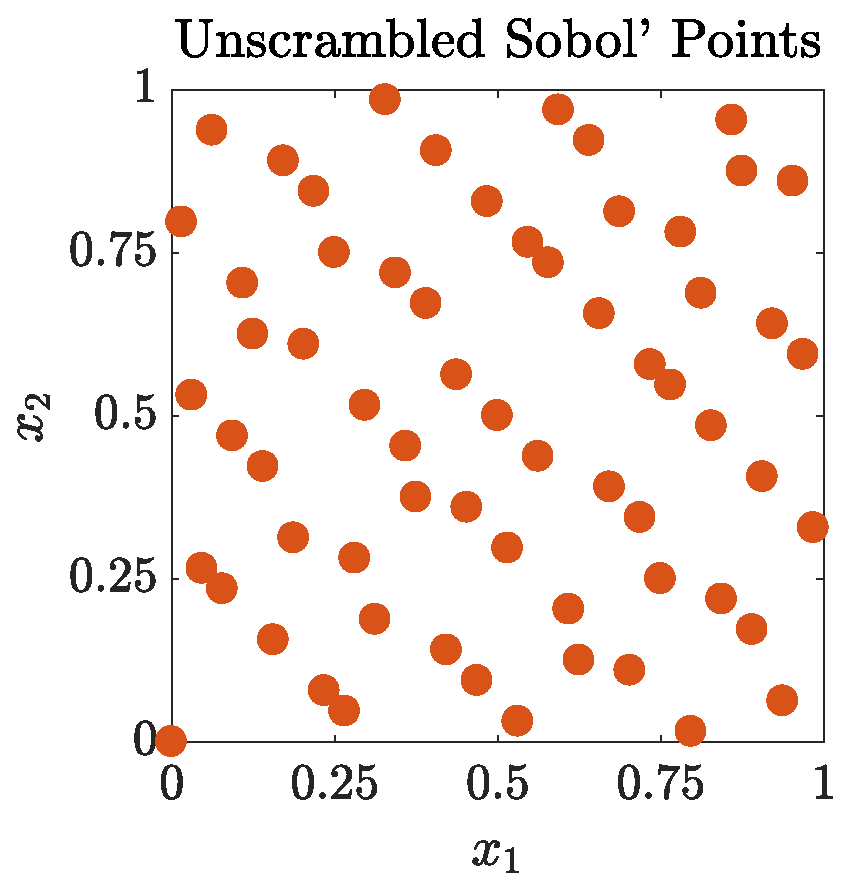
\includegraphics[height=\FJHfigheight]{ProgramsImages/USobolPoints.eps} \qquad
	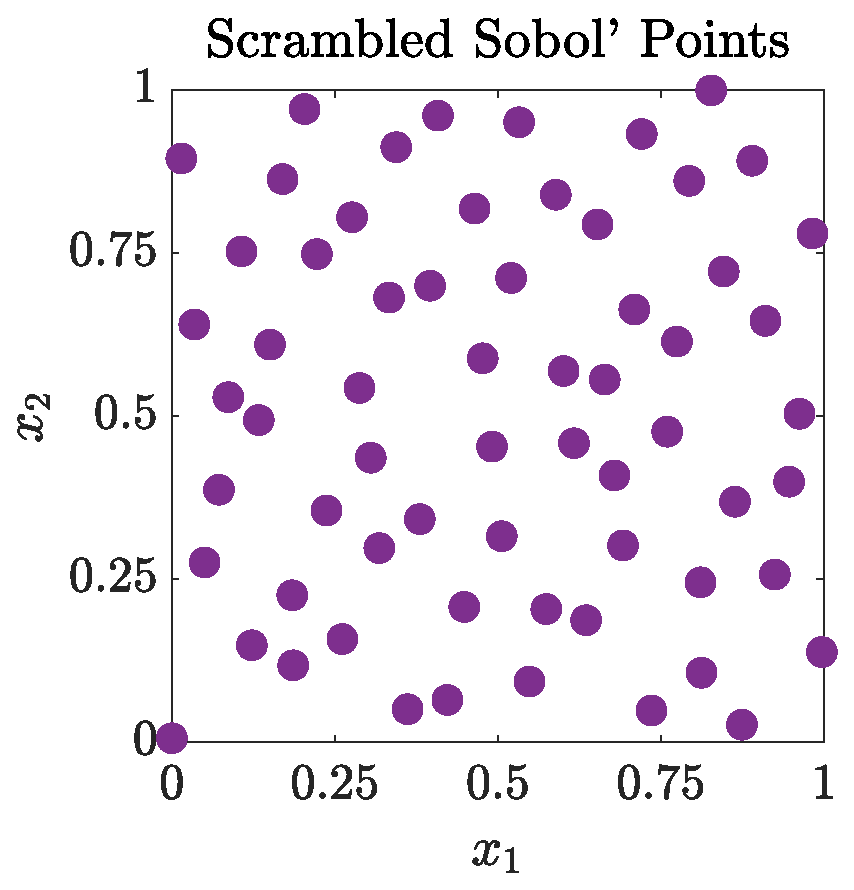
\includegraphics[height=\FJHfigheight]{ProgramsImages/SSobolPoints.eps}
	\caption{An illustration of IID points and three examples of low discrepancy points 
	\label{FJH:fig:plotsdiffpts}}
\end{figure}

\begin{figure}
	\centering
	  \includegraphics[height=\FJHfigheight]{ProgramsImages/UnwtL2Disclat.eps}   
	  \qquad 
	  \includegraphics[height=\FJHfigheight]{ProgramsImages/UnwtL2Disc.eps} 
	\caption{The root mean square $L^2$ discrepancies given by \eqref{FJH:eq:L2disc} 
	for randomly shifted 
	lattice sequence nodesets and randomly scrambled and shifted Sobol' sequences 
	points for a variety of dimensions.
		\label{FJH:fig:unwtdiscdiffpts}}
\end{figure}

\section{A Randomized Trio Identity for Cubature Error} \label{FJH:sec:rndtrio}
For the randomized version of the trio identity, we assume that the integrands lie in 
a Banach space, $(\calF,\norm{\cdot}_{\calF})$ that contains 
constant functions.  We assume
that $\int_{\calX} f(\bsx) \, \nu(\D\bsx)$ is defined  for all $f \in \calF$, however, we  
do not require 
function evaluation to be a bounded linear functional on $\calF$.  The definitions of the 
bounded linear functional $L$ and the variation in the deterministic case in  
\eqref{FJH:eq:detvardef} apply here as well.

Now endow, $\calM_{\textup{S}}$, the vector space of all sampling measures, with a 
probability distribution.  This means that the placement of the data sites, the number of 
data sites, and the choice of the weights may all be random.  We require  
the following two conditions:
\begin{subequations} \label{FJH:eq:randMcond}
\begin{gather}
\bbE_{\hnu} \biggabs{\int_{\calX} f(\bsx) \,  \hnu(\D \bsx)}^2 < \infty \qquad \forall f \in 
\calF, 
\\
\label{FJH:eq:randMcondB}
L(f) [\nu(\calX) - \hnu(\calX)] = 0  \qquad \text{almost surely}.
\end{gather}
\end{subequations}
The first condition implies that $\int_{\calX} f(\bsx) \,  \hnu(\D \bsx)$ exists 
almost surely for every $f \in \calF$.  

The randomized discrepancy is  defined as the worst  normalized root mean squared 
error:
\begin{equation} \label{FJH:eq:rnddiscdef}
\disc^\Rn(\nu - \hnu) : =\sup_{f \in \calF : f \ne 0} \frac{\displaystyle \sqrt{\bbE_{\hnu}
\biggabs{\int_{\calX} 
		f(\bsx) \, (\nu - \hnu)(\D \bsx)}^2}}{\norm{f}_{\calF}}.
\end{equation}
The randomized discrepancy does not depend on the particular instance of the 
sampling measure but on the distribution of the sampling measure. 

Finally, define the confounding as 
\begin{equation} \label{FJH:eq:rndconfdef}
\algn^\Rn(f,\nu - \hnu): =  \begin{cases} \displaystyle 
\frac{\displaystyle\int_{\calX} f(\bsx) \, (\nu - \hnu)(\D 
	\bsx)}{\Var^\Dt(f)\disc^\Rn(\nu - \hnu)},  & 
\Var^\Dt(f)\disc^\Rn(\nu - \hnu) \ne 0, \\[2ex]
0, & \text{otherwise}.
\end{cases}
\end{equation}
Here, the confounding \emph{does} depend on the particular instance of the sampling 
measure.  The above definitions allow us to establish the randomized trio identity for 
cubature 
error.

\begin{theorem}[Randomized Trio Error Identity]  \label{FJH:thm:rtrio} For the spaces of 
integrands and 
	measures defined above, and for the above definitions of variation, discrepancy, and 
	confounding, the following error identity holds for all $f \in \calF$ and $\hnu  \in 
	\calM_{\textup{S}}$: 
	\begin{equation} \tag{RTRIO} \label{FJH:eq:rtrio}
	\mu - \hmu  = \algn^\Rn(f,\nu - \hnu) \, \disc^\Rn(\nu - \hnu) \, \Var^{\Dt}(f) \quad 
	\text{almost surely}.
	\end{equation}
	Moreover, $\bbE_{\hnu} \abs{\algn^\Rn(f,\nu - \hnu)}^2  \le 1$ for all $f \in 
	\calF$. 
\end{theorem}
\begin{proof}  For all $f \in \calF$ and $\hnu  \in \calM_{\textup{S}}$, the error can be 
written as the single integral in \eqref{FJH:eq:err_as_int} almost surely. 	If $\Var^{\Dt}(f) 
= 0$, then $f = L(f)$, and $\mu - \hmu$ vanishes almost surely by
\eqref{FJH:eq:randMcondB}.  If 
$\disc^\Rn(\nu - \hnu) = 0$, then $\mu - \hmu$
	vanishes almost surely by \eqref{FJH:eq:rnddiscdef}.  Thus, for $\Var^{\Dt}(f) 
	\disc^\Rn(\nu - \hnu) = 
	0$ 
	the trio identity holds. If $\Var^{\Dt}(f) \disc^\Rn(\nu - \hnu) \ne 0$, then the trio 
	identity also holds by the definition of the confounding.
	
	Next, we analyze the magnitude of the confounding for $\Var^{\Dt}(f) \disc^\Dt(\nu - 
	\hnu) \ne 0$: 
	\begin{align*}
	\bbE \abs{\algn^\Rn(f,\nu - \hnu)}^2 & = 
	\frac{\bbE \biggl \lvert\displaystyle\int_{\calX} f(\bsx) \, (\nu - \hnu)(\D 
		\bsx) \biggr \rvert^2 }{[\Var^\Dt(f)\disc^\Dt(\nu - \hnu)]^2} \quad \text{by 
		\eqref{FJH:eq:rndconfdef}}\\
	& = \frac{\bbE \biggl \lvert\displaystyle\int_{\calX} [f(\bsx) - L(f)] \, (\nu - \hnu)(\D 
		\bsx) \biggr \rvert^2}{[\norm{f-L(f)}_{\calF}\disc^\Dt(\nu - \hnu)]^2} \quad \text{by 
		\eqref{FJH:eq:detvardef} and \eqref{FJH:eq:randMcondB}} \\
	& \le 1 \quad \text{by \eqref{FJH:eq:rnddiscdef}},
	\end{align*}
	since $\Var^{\Dt}(f) \ne 0$ and so $f - L(f) \ne 0$.
\end{proof}

Consider simple Monte Carlo, where the approximation to the integral is an equally 
weighted average using IID sampling $\bsx_1, \bsx_2, \ldots \sim 
\nu$ without 
replacement. Let the sample size be fixed at $n$.
Let $\calF = L^{2,\nu}$, the space of functions that are square integrable with respect to 
the measure $\nu$, and let $L(f)$ be the mean of $f$.  Then the variation of $f$ is just 
its standard 
deviation, $\std(f)$.  The randomized discrepancy is 
$1/\sqrt{n}$, which allows for a random sample size.  The randomized 
confounding is 
\begin{align*}
\algn^\Rn(f,\nu - \hnu) = \frac{-1}{ \sqrt{n}\, \std(f)}    \sum_{i=1}^n [f(\bsx_i) - 
\mu].
\end{align*}
This is similar to the randomized trio identity for the big data survey in 
\eqref{FJH:eq:surveyrndtrio}.

There is no simple form for the randomized discrepancy for arbitrary sampling measures 
and RKHSs like there is in the deterministic setting.  The 
randomized discrepancy can sometimes be conveniently calculated or bounded for 
spaces of integrands that are represented by series expansions, and the randomized 
sampling measures for the bases of these expansions have special properties 
\cite{HeiHicYue02a, HicWoz00a}.

It is instructive to contrast the variation, discrepancy, and confounding in the 
deterministic and randomized settings.   For some integrand, $f$, and some sampling 
measure, $\hnu$, satisfying the 
conditions defining both \eqref{FJH:eq:dtrio}  and \eqref{FJH:eq:rtrio}:
\begin{itemize}
	\item the variation in both settings is the same,
	
	\item the randomized discrepancy 
	must be no greater than the deterministic discrepancy by definition, and thus
	
	\item the randomized confounding must be no less than the deterministic 
	confounding.  
\end{itemize}
Theorem \ref{FJH:thm:dtrio} states that the deterministic confounding is never greater 
than one in magnitude.  By contrast, Theorem \ref{FJH:thm:rtrio} 
only states that the expected value of the magnitude of the randomized confounding is 
no greater than one.  The randomized confounding may be arbitrarily large, but Markov's 
inequality implies that it may be larger than $1/\sqrt{\alpha}$ with  probability no greater 
than $\alpha$.  

The big data survey example illustrated the differences in the 
deterministic and randomized trio identities.  The next example illustrates this further.

\section{Multivariate Gaussian Probabilities} \label{FJH:sec:Gauss}
Consider the $d$-variate integral corresponding to the probability of a 
$\calN(\bszero,\mathsf{\Sigma})$ random variable lying inside the box $[\bsa,\bsb]$:
\begin{equation} \label{FJH:eq:MVN}
\mu = \int_{[\bsa,\bsb]} \frac{\exp\bigl(- \frac 12 \bsz^T \mathsf{\Sigma}^{-1} \bsz 
\bigr)}{\sqrt{(2 \pi)^d \det(\mathsf{\Sigma})}} \, \D \bsz = \int_{[0,1]^{d-1}} 
f_{\textup{Genz}}(\bsx) \, \D 
\bsx,
\end{equation}
where $\mathsf{\Sigma} = \mathsf{L}\mathsf{L}^T$ is the Cholesky decomposition of 
the covariance matrix, $\mathsf{L} = \bigl(l_{jk}\bigr)_{j,k=1}^d$, is a lower triangular 
matrix, and
\begin{align}
\nonumber
\alpha_1 & = \Phi(a_1), \qquad \beta_1  = \Phi(b_1), \\
\nonumber
\alpha_j(x_1, \ldots, x_{j-1}) &= \Phi\left(\frac{1}{l_{jj}} \left(a_j - \sum_{k=1}^{j-1} 
l_{jk}\Phi^{-1}(\alpha_k + x_k(\beta_k-\alpha_k))\right)\right), \ j =2, \ldots, d,\\
\nonumber
\beta_j(x_1, \ldots, x_{j-1}) &= \Phi\left(\frac{1}{l_{jj}} \left(b_j - \sum_{k=1}^{j-1} 
l_{jk}\Phi^{-1}(\alpha_k + x_k(\beta_k-\alpha_k))\right)\right), \ j =2, \ldots, d, \\
f_{\textup{Genz}}(\bsx) &= \prod_{j=1}^{d} [\beta_j(\bsx) - \alpha_j(\bsx)]. 
\label{FJH:eq:Genz}
\end{align}
Genz \cite{Gen93} developed the clever transformation of variables above that turns the 
multivariate Gaussian probability into an integral over the unit cube.  Not only is the 
dimension decreased by one, but the integrand is typically made less peaky and more 
favorable to cubature methods.

The left plot of Fig.\ \ref{FJH:fig:MVNfig} shows the absolute errors in computing the the 
multivariate 
Gaussian probability via the Genz transformation for 
\[
   \bsa  = \begin{pmatrix}
   -6 \\ -2 \\ -2
   \end{pmatrix}, \quad
      \bsb  = \begin{pmatrix}
   5 \\ 2 \\ 1
   \end{pmatrix}, \quad
   \mathsf{\Sigma} = \begin{pmatrix} 16 & 4 & 4 \\ 4 &  2 &  1.5 \\
  4 & 1.5 &  1.3125 \end{pmatrix}, \quad
   \mathsf{L} = \begin{pmatrix} 4 & 0 & 0 \\ 1 &  1 &  0 \\
1 & 0.5 &  0.25 \end{pmatrix}, 
\]
by IID sampling, unscrambled Sobol' sequences, and scrambled Sobol' sequences   
\cite{Owe95, Owe98c}.
Multiple random scramblings of a very large scrambled Sobol' set was used to infer that 
$\mu \approx 0.6763373243578$.   For the two randomized sampling measures $100$ 
replications were taken.  The marker denotes the median error and the top of the stem 
extending above the marker denotes the worst $90\%$ error.

\begin{figure}
	\centering
	\includegraphics[height = \FJHfigheight]{ProgramsImages/MVNIIDUSobolSobol.eps} 
	\qquad 
	\includegraphics[height = \FJHfigheight]{ProgramsImages/MVNSobolGenzAff.eps}
	\caption{The error of an example of the multivariate Gaussian probability in 
	\eqref{FJH:eq:MVN}.  The left side shows the result of Genz's transformation and 
	different sampling measures.  The right side shows scrambled Sobol' sampling
	using different transformations.
	\label{FJH:fig:MVNfig}}
\end{figure}

The cubature errors for the three kinds of sampling decay at the same rates as their 
corresponding discrepancies.  The IID error tracks the rate of decay of its randomized 
discrepancy as noted above.  The cubature  error for  Sobol' 
sampling decays at the same rate as its deterministic $L^2$ discrepancy defined in 
\eqref{FJH:eq:L2disc}.  The error for randomly scrambled Sobol' 
sampling decays at a rate of roughly $\calO(n^{-3/2+\epsilon})$, which corresponds to 
the randomized discrepancy for this sampling measure \cite{HeiHicYue02a,Owe97}.  
Not only do the more evenly spaced Sobol' points improve upon IID sampling, but 
randomizing the Sobol' points while preserving their even structure provides further 
improvement to the rate of decay of the error.

The orders of the confounding in Table \ref{FJH:tab:Conf} help explain the 
benefits of randomization.  We consider cubature rules based on equally weighted 
averages of integrand values at $n$ data sites, and we consider two sample kind of 
sampling measures.  In both cases $\algn^\Rn(\nu - \hnu)$ is 
typically $\calO(1)$, but it might be much larger or smaller depending on the particular 
$\hnu$.  For IID random data sites, the 
randomized, $\disc^\Rn(\nu - \hnu) = \calO(n^{-1/2})$, as noted in Sec.\ 
\ref{FJH:sec:rndtrio}.  A poor 
arbitrary choice of data sites produces a cubature error of $\calO(1)$ because 
$\algn^\Rn(\nu - \hnu)$ is an atypically high $\calO(n^{1/2})$.  
However, both plain unscrambled Sobol', as well as scrambled Sobol' sampling yield 
atypically low $\algn^\Rn(\nu - \hnu)$ and correspondingly low cuabure errors.  For 
scrambled Sobol' sampling, the randomized discrepancy is $\disc^\Rn(\nu - \hnu) 
=\calO(n^{-3/2 + 
\epsilon})$, which is also the convergence rate for $\sqrt{\bbE_{\hnu}\bigl[\disc^\Dt(\nu - 
\hnu)\bigr ]^2}$ for scrambled 
Sobol' sampling under sufficient integrand smoothness \cite{HicHon98a, HicYue00}.
The set of all scrambled Sobol' sampling measures includes 
unscrambled 
Sobol' 
sampling, but $\algn^\Rn(\nu - \hnu)$ for unscrambled Sobol' sampling is atypically high, 
which then produces an atypically high
cubature error compared to the average for scrambled Sobol' sampling.

\begin{table}
	\caption{Confounding orders for randomized settings and 
		different sets of equi-weighted 
		sampling measures. Sufficient smoothness of the integrand is assumed.
		The order of the error equals the order of the discrepancy times the 
		order of the confounding. \label{FJH:tab:Conf}}
	\begin{equation*}
	\begin{array}{r@{\quad }c@{\quad }r@{\quad}c@{\quad}c@{\quad}c@{\quad}c}
	&&&&\text{Typical} &  \textup{Unscr.} &\text{Typical}\\
	\multicolumn{3}{r@{\quad}}{\hnu} &  \textup{Worst} &  \textup{IID} &
	\textup{Sobol'}&  \textup{Scr.\ Sobol'}\\
	\textup{Sampling Measures} & \disc^\Rn & \mu - \hmu & \calO(1) & \calO(n^{-1/2}) & 
	\calO(n^{-1+\epsilon}) & 
	\calO(n^{-3/2+\epsilon})\\
	\hline 
	\textup{IID} & \calO(n^{-1/2}) & \algn^\Rn & \calO(n^{1/2})  & \calO(1) 
	&\calO(n^{-1/2+\epsilon}) &\calO(n^{-1+\epsilon}) \\
	\textup{Scr.\ Sobol'} &\calO(n^{-3/2+\epsilon}) & \algn^\Rn 
	& & &\calO(n^{1/2+\epsilon})&\calO(1) 
	\end{array}
	\end{equation*}
\end{table}


\begin{FJHLesson}
\FJHLessonThree
\end{FJHLesson}

\begin{FJHLesson}
	\FJHLessonSeven
\end{FJHLesson}

An alternative to the Genz transformation above is an affine transformation to compute 
the multivariate Gaussian probability:
\begin{gather}
\label{FJH:eq:aff}
\bsz = \bsa + (\bsb-\bsa) \circ \bsx, \quad f_{\textup{aff}}(\bsx) =  \frac{\exp\bigl(- 
\frac 12 \bsz^T
\mathsf{\Sigma}^{-1} \bsz 
	\bigr)}{\sqrt{(2 \pi)^d \det(\mathsf{\Sigma})}} \, \prod_{j=1}^d (b_j - a_j), \\
\nonumber
\mu = 
	\int_{[0,1]^{d}} f_{\textup{aff}}(\bsx) \, \D \bsx,
\end{gather} 
where $\circ$ denotes the Hadamard (term-by-term) product.  The right plot in Fig.\ 
\ref{FJH:fig:MVNfig} shows that the error using the affine 
transformation is much worse than that using the Genz transformation even though the 
two convergence rates are the same.  Fig.\ \ref{FJH:fig:GenzAff} shows the two 
integrands.  The difference in the magnitudes of the errors is 
mainly because $\Var^{\Dt}(f_{\textup{aff}})$ is greater than 
$\Var^{\Dt}(f_{\textup{Genz}})$.


\begin{figure}
	\centering
	\includegraphics[height = \FJHfigheight]{ProgramsImages/GenzFun.eps} \qquad 
	\includegraphics[height = \FJHfigheight]{ProgramsImages/AffineFun.eps}
	\caption{Two different integrands that can be used to compute multivariate normal 
	probabilities.  The left integrand is defined in \eqref{FJH:eq:Genz}, and the right 
	integrand is defined in  \eqref{FJH:eq:aff}.
		\label{FJH:fig:GenzAff}}
\end{figure}


\begin{FJHLesson} \label{FJH:eq:lessonfour}
	\FJHLessonFour
\end{FJHLesson}


\section{Option Pricing} \label{FJH:sec:OptPrice}
The prices of financial derivatives can often be modeled by high dimensional integrals.  If 
the underlying asset is described in terms of a Brownian motion, $B$, at times $t_1, 
\ldots, t_d$, then $\bsZ = (B(t_1), \ldots, B(t_d)) \sim \calN(\bszero, \mathsf{\Sigma})$, 
where $\mathsf{\Sigma}  = \bigl( \min(t_j,t_k) \bigr)_{j,k=1}^d$, and the fair price of the 
option is
\begin{equation*}
\mu = \int_{\R^d} \textup{payoff}(\bsz) \, \frac{\exp\bigl(- \frac 12 \bsz^T 
\mathsf{\Sigma}^{-1} 
\bsz 
\bigr)}{\sqrt{(2 \pi)^d \det(\mathsf{\Sigma})}} \, \D \bsz = \int_{[0,1]^{d}} f(\bsx) \, \D \bsx 
\end{equation*}
where the function $\textup{payoff}(\cdot)$ describes the discounted payoff of the 
option, 
\begin{equation*}
f(\bsx) = \textup{payoff}(\bsz), \qquad \bsz = \mathsf{L} \begin{pmatrix}
\Phi^{-1}(x_1) \\ \vdots \\ \Phi^{-1}(x_d)
\end{pmatrix}, 
\end{equation*}
and $\mathsf{L}$ is any square matrix satisfying $\mathsf{\Sigma} = \mathsf{L} 
\mathsf{L}^T$.


Fig.\ \ref{FJH:fig:AsianOpt} shows the cubature error using IID sampling, unscrambled 
Sobol' sampling, and scrambled Sobol' sampling for the Asian arithmetic mean call option 
with the following parameters:
\begin{gather*}
\textup{payoff}(\bsz) = \max \left( \frac 1d \sum_{j=1}^d S_j - K, 0\right)\E^{-rT}, \quad
S_j = S_0 \exp\bigl( (r - \sigma^2/2) t_j + \sigma z_j\bigr),
\\
T = 1, \quad d = 12, \quad S_0 = K = 100, \quad r =  0.05, \quad \sigma = 0.5, \\
t_j = jT/d, \quad j = 1\!:\!d.
\end{gather*}
The convergence rate for IID and unscrambled Sobol' sampling are the same as in Fig.\ 
\ref{FJH:fig:MVNfig} for the previous example of multivariate probabilities.  However, 
although scrambling the Sobol' set improves the accuracy, it does not improve the 
convergence rate. 


\begin{figure}
	\centering
		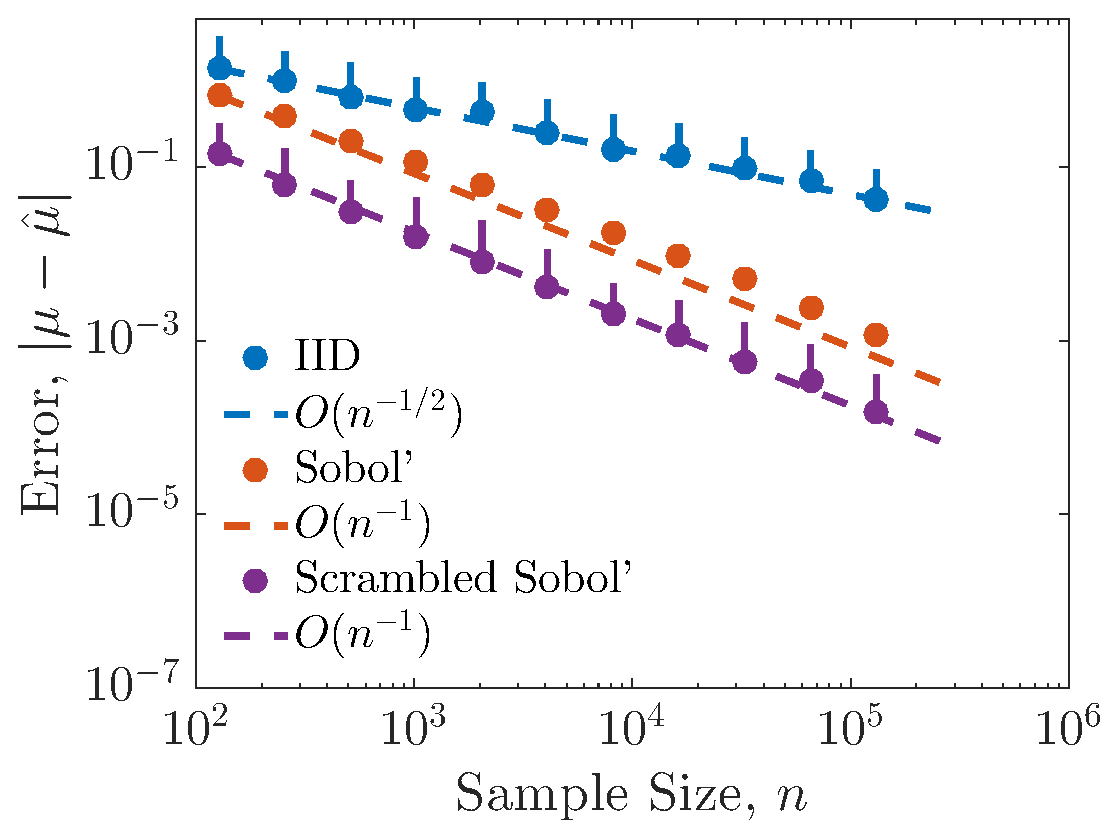
\includegraphics[height = \FJHfigheight] 
		{ProgramsImages/AsianCallIIDUSobolSobol.eps} 
		\qquad
		\includegraphics[height = \FJHfigheight] 
		{ProgramsImages/AsianCallSobolPCADiff.eps}
		\caption{Cubature error for the price of an Asian arithmetic mean option using 
		different sampling 
		measures. The left side uses the PCA decomposition and the right side contrasts 
		the PCA with the Cholesky decomposition.  \label{FJH:fig:AsianOpt}}
\end{figure}

The convergence rate for scrambled Sobol' sampling, $\hnu$,  is poorer than hoped for 
because 
$f$ is not smooth enough for $\Var^{\Dt}(f)$ to be finite in the case 
where $\disc^\Rn(\nu - \hnu) = \calO(n^{-3/2 +\epsilon})$.  Less 
stringent conditions on $f$ are required for $\disc^\Dt(\nu - \hnu) = 
\calO(n^{-1 +\epsilon})$.  Even these requirements cannot 
be ensured for option pricing examples like that above except by a rather delicate 
argument \cite{GriKuoSlo10, GriKuoSlo16}.

\begin{FJHLesson}
	\FJHLessonFive
\end{FJHLesson}

The left plot in Fig.\ \ref{FJH:fig:MVNfig} chooses $\mathsf{L} = 
\mathsf{V}\mathsf{\Lambda}^{1/2}$, where the columns of $\mathsf{V}$ are the 
eigenvectors of $\mathsf{\Sigma}$, and the diagonal elements of the diagonal matrix  
$\mathsf{\Lambda}$ are the eigenvalues of $\mathsf{\Sigma}$.  This is also called a 
principal component analysis (PCA) construction.  The advantage is that the main part of 
the 
Brownian motion affecting the option payoff is concentrated in the smaller dimensions.  
The right plot of Fig.\ 
\ref{FJH:fig:MVNfig} contrasts the cubature error for two choices of  $\mathsf{L}$:  one 
chosen by the PCA construction and the other coming from the Cholesky decomposition 
of $\mathsf{\Sigma}$.  This latter choice corresponds to constructing the Brownian 
motion by time 
differencing.  The Cholesky decomposition of $\mathsf{\Sigma}$ gives poorer rate of 
convergence, illustrating again Lesson \ref{FJH:eq:lessonfour}.


\section{A Bayesian Trio  Identity for Cubature Error} \label{FJH:sec:BayesTrio}
An alternative to the deterministic integrand considered thus far is to assume an 
integrand that is a stochastic process.  Random input functions have been hypothesized 
by 
Diaconis \cite{Dia88a}, O'Hagan \cite{OHa91a}, Ritter \cite{Rit00a}, Rasmussen and 
Ghahramani \cite{RasGha03a}, and others. Specifically, suppose that $f \sim \GP (0, 
s^2C_{\bstheta})$, a zero mean Gaussian process.  The covariance of 
this  Gaussian process is $s^2C_{\bstheta}$, where $s$ is a scale parameter, and 
$C_{\bstheta}:\calX \times \calX \to \R$ is defined by a shape parameter $\bstheta$.  
The 
sample space for this Gaussian process, $\calF$, does not enter significantly into the 
analysis.  Define the vector space of measures 
\begin{equation*}
\calM = \left\{\eta :  \int_{\calX^2} C_\bstheta(\bsx,\bst) 
\, \eta(\D \bsx) \eta(\D \bst) < \infty, \ \ \int_{\calX^2} C_\bstheta(\bsx,\bst) 
\, \eta(\D \bsx) < \infty \ \ \forall \bst \in \calX \right \},
\end{equation*}
and let $C_{\bstheta}$ be such that $\calM$ contains both $\nu$ and the Dirac 
measures 
$\delta_{\bst}$ for all $\bst \in \calX$. 

For a Gaussian process, all vectors of linear functionals of $f$ have a multivariate 
Gaussian distribution.  It then follows that for a 
deterministic sampling measure, $\hnu = \sum_{i=1}^n w_i \delta_{\bsx_i}$, the cubature 
error, $\mu - \hmu$, is distributed as $\calN \bigl(0 , s^2(c_0 - 
2 \bsc^T \bsw + \bsw ^T \mC \bsw) \bigr)$, where 
\begin{subequations} \label{FJH:eq:Cvecmatdef}
\begin{gather}
c_0  = \int_{\calX^2} C_\bstheta(\bsx,\bst) \, \nu(\D \bsx) \nu(\D \bst), \qquad \bsc = 
\biggl( 
\int_{\calX} 
C_\bstheta(\bsx_i,\bst) \,\nu(\D \bst) \biggr)_{i=1}^n, \\
\mC  = \bigl( C_\bstheta(\bsx_i,\bsx_j) \bigr)_{i,j=1}^n, \qquad \bsw = \bigl(w_i 
\bigr)_{i=1}^n.
\end{gather}
\end{subequations}
The dependence of $c_0$, $\bsc$, and $\mC$ on $\bstheta$ is suppressed in the 
notation for simplicity. We 
define the Bayesian variation, discrepancy and confounding as 
\begin{subequations} \label{FJH:eq:btriodef}
\begin{gather}
\label{FJH:eq:btriodefa}
\Var^{\Ba}(f)  = s, \qquad \disc^{\Ba}(\nu - \hnu) = \sqrt{c_0 - 
	2 \bsc^T \bsw + \bsw ^T \mC \bsw},\\
\algn^{\Ba}(f,\nu - \hnu) :=\frac{ \int_{\calX} 
	f(\bsx) \, (\nu - \hnu)(\D\bsx)}{s \sqrt{c_0 - 2 \bsc^T \bsw + \bsw ^T \mC \bsw}}.
\end{gather}
\end{subequations}

\begin{theorem}[Bayesian Trio Error Identity]  \label{FJH:thm:btrio} Let the integrand be 
an instance of a zero mean Gaussian process with covariance $s^2C_{\bstheta}$ and 
that is drawn from a sample space 
$\calF$.  For the  variation, discrepancy, and 
	confounding defined in \eqref{FJH:eq:btriodef}, the following error identity holds: 
	\begin{equation} \tag{BTRIO} \label{FJH:eq:btrio}
	\mu - \hmu  = \algn^\Ba(f,\nu - \hnu) \, \disc^\Ba(\nu - \hnu) \, \Var^{\Ba}(f) \quad 
	\text{almost surely}.
	\end{equation}
	Moreover, $\algn^\Ba(f,\nu - \hnu) \sim \calN(0,1)$. 
\end{theorem}
\begin{proof}  Although $\int_{\calX} f(\bsx) \, \nu(\D \bsx)$ and $f(\bst) = \int_{\calX} 
f(\bsx) \, \delta_\bst (\D \bsx)$ may not exist for all $f \in \calF$, these two quantities 
exist 
almost surely because $\bbE_f [\int_{\calX} f(\bsx) \, \nu(\D \bsx)]^2 = c_0$, and 
$\bbE_f [f(\bsx)]^2 = C(\bsx,\bsx)$ are both well-defined and finite.  The proof of the 
Bayesian trio identity follows directly from the definitions above.  The 
distribution of the confounding follows from the distribution of the cubature error.
\end{proof}

The choice of cubature weights that 
minimizes the Bayesian discrepancy in \eqref{FJH:eq:btriodefa} is $\bsw = 
\mathsf{C}^{-1} \bsc$, which results in $\disc^{\Ba}(\nu - \hnu) = \sqrt{c_0 - \bsc ^T 
\mC^{-1} \bsc}$ and $\mu - \hmu \sim \calN \bigl(0 , s^2(c_0 - \bsc ^T 
\mC^{-1} \bsc) \bigr)$.  However, computing the weights requires $\calO(n^3)$ 
operations 
unless $\mathsf{C}$ has some special structure.  This computational cost is significant 
and may be a deterrent to the use of optimal weights unless the weights are 
precomputed. For smoother covariance functions, $C_\bstheta$, there is often a 
challenge of $\mathsf{C}$ being ill-conditioned.

The \emph{conditional} distribution of the cubature error, $\mu - \hmu$, given the 
observed data $ \{f(\bsx_i )= y_i\}_{i=1}^n$ is $\calN \bigl( \bsy^T (\mC^{-1}\bsc - 
\bsw) , s^2(c_0 - \bsc ^T \mC^{-1} \bsc) \bigr)$.  To remove the bias one should again 
choose $\bsw = \mathsf{C}^{-1} \bsc$.  This also makes the conditional distribution of 
the cubature error the same as the unconditional distribution of the cubature error.

Because the cubature error is a normal random variable, we may use function 
values perform useful inference, namely, 
\begin{equation} \label{FJH:eq:MLEBdOne}
\bbP_f\bigl[\abs{\mu - \hmu} \le 2.58 
\disc^{\Ba}(\nu - \hnu) \Var^{\Ba}(f)\bigr] = 99\%.
\end{equation}
However, unlike our use of random sampling measures that are drawn via carefully 
crafted random number generators, there is no assurance that our integrand is actually 
drawn from a Gaussian process whose covariance we have fixed in advanced.  

The covariance, $s^2 C_{\bstheta}$, should be estimated, and one way to do so is 
through 
maximum likelihood estimation (MLE), using the function values drawn for the purpose of 
estimating the integral.  The log-likelihood function for the data $ \{f(\bsx_i )= 
y_i\}_{i=1}^n$ is
\begin{align*}
\ell(s,\bstheta | \bsy) & = \log \left(\frac{\exp\left(- \frac 12 s^{-2} \bsy^T 
\mathsf{C_{\bstheta}}^{-1} \bsy\right)}{\sqrt{(2\pi)^n  \det(s^2 
\mathsf{C_{\bstheta}})}}\right)\\
& = - \frac 12 s^{-2} \bsy^T \mathsf{C_{\bstheta}}^{-1} \bsy -\frac 12  
\log \bigl(
\det(\mathsf{C_{\bstheta}}) \bigr) - \frac n2 \log(s^2) + \text{constants}.
\end{align*}
Maximizing with respect to $s^2$, yields the MLE scale parameter:
\[
s_\MLE =  \sqrt{\frac 1n \bsy^T \mathsf{C_{\bstheta_\MLE}}^{-1} \bsy}.
\]
Plugging this into the log likelihood leads to the MLE shape parameter: 
\[
\bstheta_\MLE =  \argmin_\bstheta \left[\frac 1n \log \bigl(\det(\mathsf{C_{\bstheta}}) 
\bigr) 
+ \log\bigl(\bsy^T \mathsf{C_{\bstheta}}^{-1} \bsy \bigr)  \right ],
\]
which requires numerical optimization to evaluate. Using MLE estimates, the probabilistic 
error 
bound in \eqref{FJH:eq:MLEBdOne} becomes
\begin{multline} \label{FJH:eq:MLEBdTwo}
\bbP_f\left[\abs{\mu - \hmu} \le 2.58 
\sqrt{\frac 1n \left(c_{0,\bstheta_\MLE} - \bsc_{\bstheta_\MLE} ^T 
	\mC_{\bstheta_\MLE}^{-1} \bsc_{\bstheta_\MLE} \right)  \left(\bsy^T 
	\mathsf{C}_{\bstheta_\MLE}^{-1} \bsy\right)}\right] \\
 = 99\%.
\end{multline}
Note that the value of $\bstheta_\MLE$ and the above Bayesian cubature error bounds  
is unchanged by replacing  $C_\bstheta$ by a positive multiple of itself.  

Let's revisit the multivariate normal probability example of Sec.\ \ref{FJH:sec:Gauss}, 
and perform Bayesian cubature with a covariance kernel with modest smoothness from 
the Mat\'ern  family:
\begin{equation} \label{FJH:eq:Matern}
C_\theta(\bsx,\bst) = \prod_{j=1}^d \left(1 + 
\theta\abs{x_j-t_j}\right) \exp\left(-\theta\abs{x_j-t_j}\right)
\end{equation}
A two-dimensional example of this covariance kernel is plotted in Fig.\ 
\ref{FJH:fig:MVNcubMLE}.  Using $100$ randomly scrambled Sobol' samples, the 
Bayesian 
cubature method outlined above was used to compute the multivariate normal probability 
$\mu$.  The scale and shape parameters were estimated by MLE, and the optimal 
cubature weights $\bsw = 
\mathsf{C}_{\theta_{\MLE}}^{-1} \bsc_{\theta_{\MLE}}$ were used to compute $\hmu$.  
The actual errors are plotted in Fig.\ \ref{FJH:fig:MVNcubMLE}, which also provides a 
contrast of the actual error and the probabilistic error bound.  This bound was correct 
about $83\%$ of the time.  Based on the smoothness of the integrand and the kernel, 
one might expect $\calO(n^{-2})$ convergence of the answer, but this is not clear from 
the numerical computations.

\begin{figure}
	\centering
		\includegraphics[height = \FJHfigheight] 
{ProgramsImages/Matern.eps} 
\\[2ex]
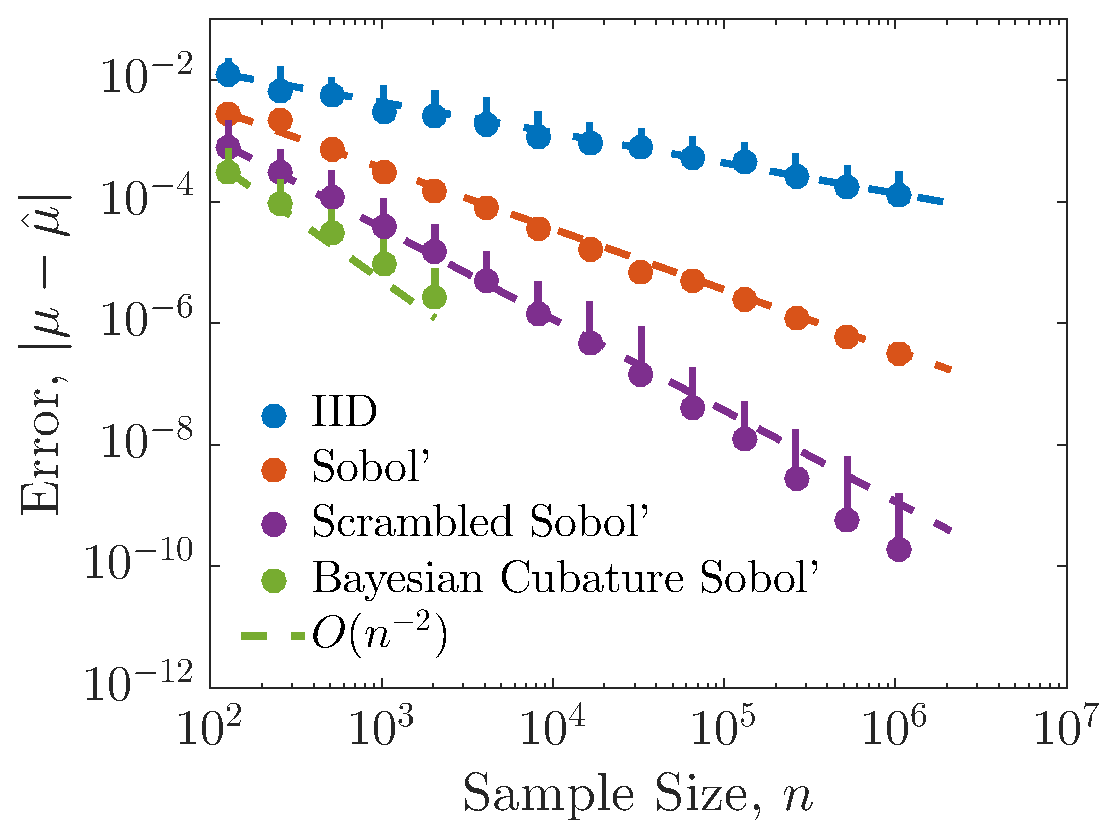
\includegraphics[height = \FJHfigheight] 
{ProgramsImages/MVNIIDUSobolSobolWtSobol.eps}
\qquad
\includegraphics[height = \FJHfigheight] 
{ProgramsImages/MVNSobolWtSobolErrBd.eps}
\caption{The Mat\'ern kernel in \eqref{FJH:eq:Matern} (top), the cubature errors for the 
multivariate normal 
proabability example using Bayesian cubature (bottom left), and the Bayesian cubature 
error versus the probabilistic error bound in \eqref{FJH:eq:MLEBdTwo} (bottom right). 
\label{FJH:fig:MVNcubMLE}}
\end{figure}

\begin{FJHLesson}
	\FJHLessonTen
\end{FJHLesson}

Bayesian cubature offers hope with a dose of caution.  The theory is solid, but as  this 
example shows, one cannot know if the actual integrand under consideration is a typical 
instance of the Gaussian process being assumed, even using MLE to determine the 
parameters of the distribution.  The success rate of the probabilistic error bound for this 
example is high, but not as high as the theory would suggest.  One may ask whether a 
larger candidate family of Gaussian processes needs to be considered, but then this 
would increase 
the time required for estimation of the parameters.  Even now, this example was carried 
out to only a rather modest sample size because of the $\calO(n^3)$ operations 
required to compute each $\hmu$.  Efforts to reduce this operation count have been 
made by Anitescu, Chen, and Stein \cite{AniCheSte16a}, Parker, Reich and Gotwalt 
\cite{ParEtal17a}, and others.  Probabilistic numerics, 
\url{http://www.probabilistic-numerics.org}, of which Bayesian cubature is an example, 
holds promise that deserves further exploration.


\section{A Deterministic Interpretation of Bayesian Cubature} 
\label{FJH:sec:DetBayesInterp}
The advantage of the Bayesian approach is that there is an upper bound on the cubature 
error that depends on the function data obtained in the process of computing $\hmu$ 
(see \eqref{FJH:eq:MLEBdTwo}), an not on an unknown norm of the integrand as is the 
case with $\Var^{\Dt}(f)$.  This raises the question of whether one can interpret 
Bayesian cubature in a deterministic way.  We have not seen such an interpretation in 
the literature, but we provide one here.

Suppose that integrands lie in Hilbert space,  $\calF$, with reproducing kernel 
$K_\bstheta$, that is defined identically to the covariance function 
$C_\bstheta$ used in Bayesian cubature.  Let $L(f)$ be identically zero, 
so that $\Var^{\Dt}(f) = \norm{f}_{\calF}$.  Define the scalar $k_0$, the vector $\bsk$, 
and the matrix $\mathsf{K}$ analogously to $c_0$, $\bsc$, and $\mathsf{C}$, 
respectively, as in  \eqref{FJH:eq:Cvecmatdef}.  Let the cubature weights be $\bsw = 
\mathsf{K}^{-1} \bsk$, analogous to what is done for Bayesian cubature.  This means 
that $\disc^\Dt(\nu - \hnu)$ is numerically the same as $\disc^\Ba(\nu - \hnu)$.

\begin{FJHLesson}
	\FJHLessonFourteen
\end{FJHLesson}

The minimum Hilbert space norm 
interpolant of $f \in \calF$ given the data $ \{f(\bsx_i )= y_i\}_{i=1}^n$ is $\tf_\bsy(\bsx) = 
\tbsk(\bsx) \mathsf{K}^{-1} \bsy$, where $\tbsk(\bsx) := 
\bigl( K_\bstheta(\bsx_i,\bsx) \bigr)_{i=1}^n$.  Moreover, $\norm{\tf_\bsy}^2_{\calF} = 
\bsy^T 
\mathsf{K}^{-1} \bsy$.  Thus, in the deterministic Hilbert space setting, the probabilistic 
Bayesian cubature error bound \eqref{FJH:eq:MLEBdTwo} is translated as
\begin{equation} \label{FJH:eq:BaysDetBdOne}
\abs{\mu - \hmu} \le \frac{2.58}{\sqrt{n}} \disc^{\Dt}(\nu - \hnu) \Var^{\Dt}(\tf_\bsy)  
\qquad \text{for } f\in \calT.
\end{equation}
Here the ``$99\%$ probability'' statement in the Bayesian setting is replaced by requiring 
$f$ to lie in a set $\calT$ of \emph{typical} integrands. 

To define $\calT$ precisely, we note that the choice of cubature weights $\bsw = 
\mathsf{K}^{-1} \bsk$ not only minimizes the deterministic discrepancy, it also 
corresponds to the approximation $\hmu= \int_{\calX} \tf_\bsy(\bsx) \, \nu(\D \bsx)$.  
Therefore, the deterministic trio identity, \eqref{FJH:eq:dtrio}, implies that  
\begin{align*}
\mu - \hmu & = \mu(f - \tf_\bsy) = \mu(f - \tf_\bsy) - \hmu(f - \tf_\bsy) \\
& = \algn^{\Dt}(f - 
\tf_\bsy,\nu - \hnu) \disc^\Dt(\nu - \hnu) \Var^\Dt(f - \tf_\bsy),
\end{align*}
where the notation $\mu(\cdot)$ is used to specify the integrand explicitly. Since 
$\abs{\algn^{\Dt}(f - 
	\tf_\bsy,\nu - \hnu)} \le 1$, this means that \eqref{FJH:eq:BaysDetBdOne} is true for 
	$\Var^\Dt(f - \tf_\bsy) \le 2.58 \Var^{\Dt}(\tf_\bsy) /\sqrt{n}$. For a
RKHSs, $[\Var^\Dt(f)]^2 = [\Var^\Dt(\tf_\bsy)]^2 + 
[\Var^\Dt(f - \tf_\bsy)]^2$, which implies that \eqref{FJH:eq:BaysDetBdOne} is true for 
\begin{equation*}
\calT := \left \{f \in \calF : \Var^\Dt(f - \tf_\bsy) \le \frac{2.58}{\sqrt{n + 2.58^2}} 
\Var^{\Dt}(f) 
\right\} .
\end{equation*}
Integrands in $\calT$ are well approximated by their minimum norm interpolants.  We 
note that the definition of $\calT$ 
depends on $\hnu$, which seems unavoidable.

There still remains the matter of interpreting the MLE estimate of $\bstheta$ 
deterministically.  Consider the ellipsoid defined as all possible function data for 
which the minimum norm approximation has a smaller norm than that observed:
\[
\calE_\bstheta = \left\{ \bsz \in \R^n :  \bsz^T 
\mathsf{K}_\bstheta^{-1} \bsz = \norm{\tf_\bsz}_{\calF_\bstheta} \le 
\norm{\tf_\bsy}_{\calF_\bstheta} =  \bsy^T 
\mathsf{K}_\bstheta^{-1} \bsy \right\}.
\]
The volume of this ellipsoid is proportional to $\sqrt{\det(\mathsf{K}_\bstheta) [ \bsy^T 
	\mathsf{K}_\bstheta^{-1} \bsy]^n}$.  Choosing the value of $\bstheta$ that minimizes 
	the volume of this ellipsoid is equivalent to the definition of $\bstheta_\MLE$ with 
	$C_\bstheta$ replaced by $K_\bstheta$.  This provides a determnistic interpretation of 
	the best choice of the shape parameter.
	
\begin{FJHLesson}
	\FJHLessonNine
\end{FJHLesson}

\section{A Randomized Bayesian Trio Identity for Cubature Error}

So far, we have presented three versions of the trio identity: a deterministic verion  in 
Theorem \ref{FJH:thm:dtrio}, a randomzied version in Theorem \ref{FJH:thm:rtrio}, and a 
Bayesian 
version in Theorem \ref{FJH:thm:btrio}.  The fourth and final version is a randomized 
Bayesian trio identity.  The variation remains unchanged from the Bayesian definition in 
\eqref{FJH:eq:btriodefa}.  
The randomized Bayesian discrepancy and confounding are defined as follows:
\begin{subequations} \label{FJH:eq:rbtriodef}
	\begin{gather}
	\label{FJH:eq:bbtriodefa}
\disc^{\Rn\Ba}(\nu - \hnu) = \sqrt{\bbE_{\hnu}  \bigl(c_0 - 
		2 \bsc^T \bsw + \bsw ^T \mC \bsw \bigr)},\\
	\algn^{\Rn\Ba}(f,\nu - \hnu) :=\frac{ \int_{\calX} 
		f(\bsx) \, (\nu - \hnu)(\D\bsx)}{s  \sqrt{\bbE_{\hnu}  \bigl(c_0 - 
			2 \bsc^T \bsw + \bsw ^T \mC \bsw \bigr)}}.
	\end{gather}
\end{subequations}
The proof of the randomized Bayesian trio error identity is similar to the proofs of the 
other trio identities and is omitted.

\begin{theorem}[Randomized Bayesian Trio Error Identity]  \label{FJH:thm:rbtrio} Let 
the integrand be 
	an instance of a zero mean Gaussian process with covariance $s^2C_{\bstheta}$ and 
	that is drawn from a sample space $\calF$.  Let the sampling measure be drawn 
	randomly from $\calM_{\textup{S}}$ according to some probability distribution.  For 
	the  
	variation defined in \eqref{FJH:eq:btriodefa}, and the discrepancy and 
	confounding defined in \eqref{FJH:eq:rbtriodef}, the following error identity holds: 
	\begin{equation} \tag{RBTRIO} \label{FJH:eq:rbtrio}
	\mu - \hmu  = \algn^{\Rn\Ba}(f,\nu - \hnu) \, \disc^{\Rn\Ba}(\nu - \hnu) \, \Var^{\Ba}(f) 
	\quad 
	\text{almost surely}.
	\end{equation}
	Moreover, $\algn^{\Rn\Ba}(f,\nu - \hnu) \sim \calN(0,1)$. 
\end{theorem}

\begin{FJHLesson}
	\FJHLessonSix
\end{FJHLesson}

When the cubature weights are all equal to $1/n$, i.e., $\bsw = \bsone/n$, then it is 
often possible to compute 
$\disc^{\Rn\Ba}(\nu - \hnu)$ in terms of the Bayesian discrepancy for a filtered kernel 
when the randomized data sites satisfy a natural 
property.  Suppose that $\bsx_i =\bspsi (\bsz_i)$ for $i = 1 \!:\!n$, where 
$\{\bsz_i\}_{i=1}^n$ are deterministic data sites, and $\bspsi :\calX \to \calX$ is a random 
function.  For example, for IID sampling on $\calX$, $\bspsi(\bsx) = \bsDelta_\bsx$, 
where 
$\bsDelta_\bsx$ is a random point distributed according to $\nu$ and depending on 
$\bsx$.  For uniform random shifts modulo $\bsone$ on the unit cube, 
which are applied to nodesets of lattices, $\bspsi(\bsx) = \bsx + \bsDelta \bmod \bsone$, 
where $\bsDelta \sim \calU[0,1]^d$.  For randomly scrambled digital sequences there 
also 
exists such a $\bspsi$, but its definition is more complex.  Furthermore, assume that for 
any IID random variables $\bsX, \bsZ \sim \nu$,  the random variables $\bspsi(\bsX), 
\bspsi(\bsZ)$ are also IID with probability measure $\nu$.  In addition, for any $(\bsx, 
\bst) \in \calX \times \calX$ suppose that  $\bigl(\bspsi(\bsx), \bspsi(\bst) \bigr)$ and 
$\bigl(\bspsi(\bspsi(\bsx)), \bspsi(\bspsi(\bst)) \bigr)$ have the same probability measure.

Define a filtered version of the covariance kernel as $\filC(\bsx,\bst) = \bbE_{\bspsi} 
C\bigl(\bspsi(\bsx), \bspsi(\bst) \bigr)$.  Here the dependence on $\bstheta$ is 
suppressed.  Then the terms that comprise randomized 
Bayesian discrepancy are
%\begin{subequations} \label{FJH:eq:filCvecmatdef}
	\begin{gather*}
	 \bbE_{\bspsi}(c_0)  = c_0 =  \int_{\calX^2} C(\bsx,\bst) \, \nu(\D \bsx) \nu(\D 
	 \bst) = 
	 \int_{\calX^2} \filC(\bsx,\bst) \, \nu(\D \bsx) \nu(\D \bst) =: \filc_0, \\
	 \bbE_{\bspsi}(\bsc) = 
	\biggl( \int_{\calX} 
	\bbE_{\bspsi}\bigl[C(\bspsi(\bsz_i),\bst)] \,\nu(\D \bst) \biggr)_{i=1}^n = 
	\biggl( \int_{\calX} 
	\filC(\bsz_i,\bst) \,\nu(\D \bst) \biggr)_{i=1}^n = : \filbsc, \\
	 \bbE_{\bspsi}(\mC)  = \biggl(  \bbE_{\bspsi} 
	 C\bigl(\bspsi(\bsz_i), \bspsi(\bsz_j) \bigr) \biggr)_{i,j=1}^n = \Bigl( \filC(\bsz_i,\bsz_j) 
	 \Bigr)_{i,j=1}^n =: \filmC.
	\end{gather*}
%\end{subequations}
Thus, the randomized Bayesian discrepancy based on the kernel $C$ with random data 
sites $\{\bsx_i = \bspsi(\bsz_i)\}_{i=1}^n$ is the same as the Bayesian discrepancy based 
on the filtered kernel, $\filC$, with deterministic data sites $\{\bsz_i\}_{i=1}^n$.  That is, 
\begin{multline}
\disc^{\Rn\Ba}\biggl(\nu - \frac 1n \sum_{i=1}^n \delta_{\bspsi(\bsz_i)} ; C\biggr) = 
\disc^{\Rn\Ba}\biggl(\nu - \frac 1n \sum_{i=1}^n \delta_{\bspsi(\bsz_i)} ; \filC\biggr) \\
=
\disc^{\Ba}\biggl(\nu - 
\frac 1n \sum_{i=1}^n \delta_{\bsz_i} ; \filC \biggr)
\end{multline}
This relationship is often used to determine the decay of the discrepancies of 
randomized low 
discrepancy data sites (see e.g., \cite{HicWoz00a, HicYue00}).

It was noted in Sec.\ \ref{FJH:sec:DetBayesInterp} that when the reproducing kernel, 
$K$, in the deterministic setting is numerically the same as the covariance kernel, $C$, 
in the Bayesian setting, then $\disc^\Dt(\nu - \hnu)$ is numerically the same as 
$\disc^\Ba(\nu - \hnu)$.  This equality extends to the randomized setting in that 
\begin{equation*}
\bigl[\disc^{\Rn}(\nu - \hnu)\bigr]^2 \le \bbE_{\hnu} \bigl[\disc^\Dt(\nu - \hnu)\bigr]^2 = 
\bbE_{\hnu} \bigl[\disc^\Ba(\nu - 
\hnu)\bigr]^2 = \bigl[\disc^{\Rn\Ba}(\nu - \hnu)\bigr]^2.
\end{equation*}

\section{Dimension Dependence of the Cubature Error and Discrepancy} 
\label{FJH:sec:Tract}
The statements about the rates of decay of discrepancy and cubature error as the 
sample size increases have so far ignored the dependence on the dimension of the 
integration domain.  On the one hand, Fig.\ \ref{FJH:fig:AsianOpt} on the left shows a 
clear error 
decay rate of $\calO(n^{-1 + \epsilon})$ for low discrepancy sampling for the option 
pricing problem with dimension $12$.  However, Fig.\ \ref{FJH:fig:unwtdiscdiffpts} shows 
that the discrepancy for these scrambled Sobol' points does not decay like $\calO(n^{-1 
+ \epsilon})$ for moderate $n$.  

There has been a tremendous effort to 
understand the effect of the dimension of the integration problem on the convergence 
rate.  Sloan and Wo\'zniakowski \cite{SloWoz97} pointed out how
the sample size required to achieve a desired error tolerance could grow exponentially 
with 
dimension.  Such problems are called \emph{intractable}.  This led to a search for 
settings where the sample size required to attain achieve a desired error tolerance only 
grows polynomially with dimension (\emph{tractable} problems) or is independent of the 
dimension (\emph{strongly tractable} problems). The three volume masterpiece by Novak 
and Wo\'zniakowski \cite{NovWoz08a,NovWoz10a,NovWoz12a} and the references cited 
therein contain necessary and sufficient conditions for tractability.  A parallel idea is that 
of \emph{effective dimension}, introduced by Caflisch, Morokoff, 
and Owen \cite{CafMorOwe97} and developed further in \cite{LiuOwe04a}.

Here we provide a glimpse into those situations where the dimension of the problem does 
not have an adverse effect on the convergence rate of the cubature error and the 
discrepancy.  Let's generalize the reproducing kernel used to define the 
$L^2$ discrepancy in \eqref{FJH:eq:L2Kdef}, as well as the corresponding 
variation and the discrepancy for equi-weighted sampling measures:
\begin{gather*} \label{FJH:eq:wtL2Kdef}
K(\bsx,\bst) =\prod_{k = 1}^d [1 + \gamma_k^2\{1 - \max(x_k,t_k)\}], \\
\Var^\Dt(f) = \Bigl \lVert \bigl (\gamma_{\fraku}^{-1}
\lVert\partial^{\fraku} f\rVert_{L^2}\bigr )_{\fraku \ne \emptyset} \Bigr \rVert_2 \qquad
\gamma_{\fraku} = \prod_{k \in \fraku} \gamma_k,
\end{gather*}
\begin{multline} \label{FJH:eq:wtL2disc}
\bigl[\disc^\Dt(\nu - \hnu)\bigr]^2 = \prod_{k=1}^d\Bigl(1 + \frac{\gamma_k^2}{3}\Bigr)
- \frac{2}{n} \sum_{i=1}^n \prod_{k=1}^d \left (1 + \frac{\gamma_k^2(1 - 
x_{ik}^2)}{2} \right) \\ + \frac{1}{n^2}\sum_{i,j=1}^n \prod_{k = 1}^d [1 + 
\gamma_k^2( 1 - \max(x_{ik},x_{jk}))]
\end{multline}
For $\gamma_1 = \cdots = \gamma_d = 1$, we recover the situation in Sec.\ 
\ref{FJH:sec:dettrio}, where the decay rate of the discrepancy was dimension dependent 
for moderate sample sizes.  However if $\gamma_k^2 = 
k^{-3}$, then the discrepancies for randomly shifted lattice nodesets and scrambled   
Sobol' sequences show only a slight dimension dependence, as shown in Fig.\ 
\ref{FJH:fig:wtdiscdiffpts}.

\begin{figure}
	\centering
	\includegraphics[height=\FJHfigheight]{ProgramsImages/WtL2Disclat.eps}   \qquad 
	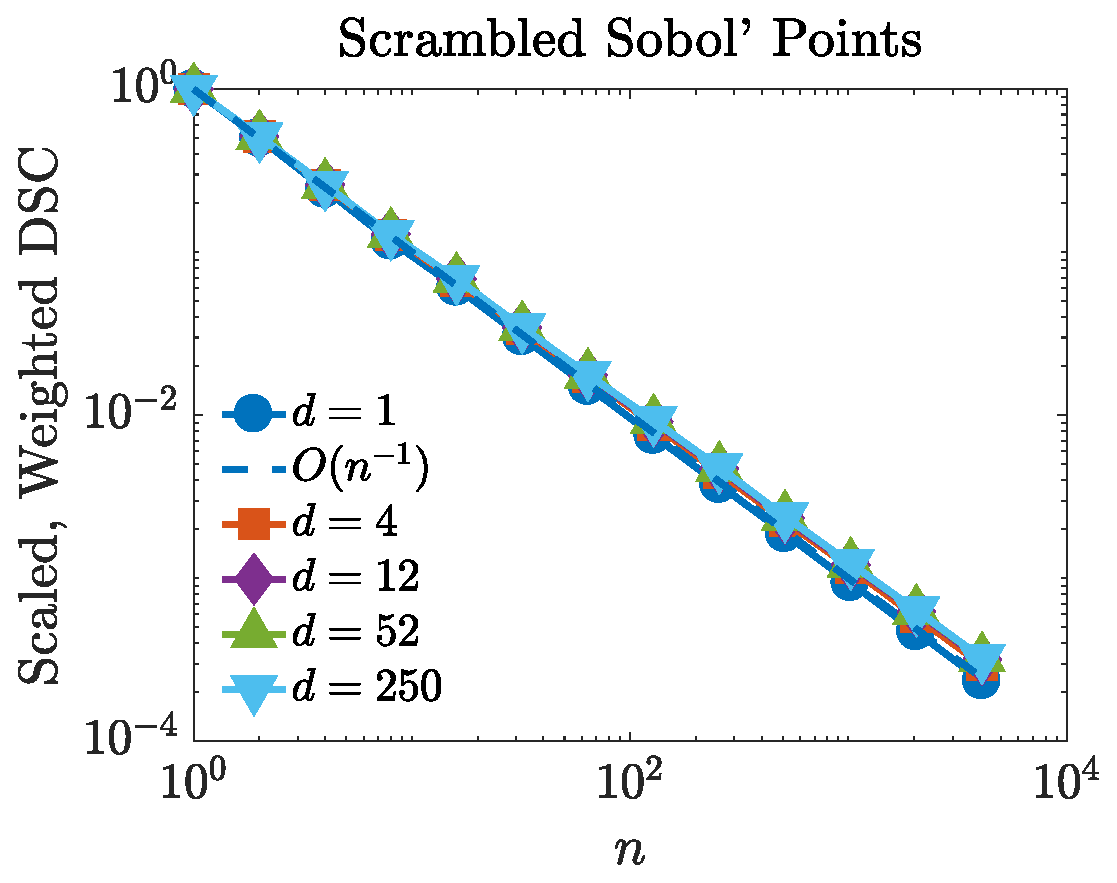
\includegraphics[height=\FJHfigheight]{ProgramsImages/WtL2Disc.eps} 
	\caption{The root mean square weighted $L^2$ discrepancies given by 
	\eqref{FJH:eq:wtL2disc} 
		for randomly shifted 
		lattice sequence nodesets and randomly scrambled and shifted Sobol' sequences 
		points.  A variety of dimensions are shown.
		\label{FJH:fig:wtdiscdiffpts}}
\end{figure}

When the weights $\gamma_k$ decay with $k$, the discrepancy depends \emph{less} 
on how evenly the data sites appear in projections involving the higher coordinates.  On 
the other hand, the variation in this case gives 
\emph{heavier} weight to the $\partial^{\fraku} f$ with 
$\fraku$ involving large $k$.  For the cubature error decay to mirror the decay of the 
discrepancy shown in Fig.\ \ref{FJH:fig:wtdiscdiffpts}, the integrand must depend only 
slightly on the coordinates with higher indices, so that the variation will be modest.

\begin{FJHLesson}
	\FJHLessonEight
\end{FJHLesson}

\section{Rewriting the Integral}

The same integral $\mu$ can often written in multiple ways by making variable 
transformations.  This can be advantageous if a variable transformation reduces the 
variation of the integrand.  An example of this is shown in Fig.\ \ref{FJH:fig:GenzAff} for 
computing the multivariate normal probability in Sec.\ \ref{FJH:sec:Gauss}.  Another 
example is shown in Fig.\ \ref{FJH:fig:AsianOpt} for computing option prices  in Sec.\ 
\ref{FJH:sec:OptPrice}.  In that example, the preferred variable transformation causes 
the integrand to depend less on the higher numbered coordinates, which fits the situation 
described in the previous section where the discrepancy and cubature error become 
nearly dimension-independent when the variance defined in terms of decreasing 
coordinate weights also be comes dimension-independent.

Importance sampling is a way to improve the accuracy of IID Monte Carlo 
methods, but it can also be useful for quasi-Monte Carlo methods, which are based on 
low discrepancy sequences.  Since low discrepancy sampling measures are essentially 
always generated to mimic the uniform measure on the unit cube, $[0,1]^d$, the final 
integral \eqref{FJH:eq:INT} should essentially end up as $\mu = \int_{[0,1]^{d}} f(\bsx) \, 
\D\bsx$.  Suppose that one starts with $\mu = \int_{\calX} g(\bst) \, 
\D\bst$ and can identify an onto mapping $\bszeta: [0,1]^d \to \calX$ with finite
Jacobian $\det\bigl( \partial \bszeta/\partial \bsx\bigr)$.  Then these two expressions for 
$\mu$ coincide provided that $f(\bsx) = g(\bszeta(\bsx)) \det\bigl( \partial 
\bszeta/\partial \bsx\bigr)$.  Since the choice of $\bszeta$ is not unique, it should be 
chosen to make $\Var^\Dt(f)$ as small as possible, which is more of an art than a 
science.

Control variates can be used to make the variation of the integrand smaller for 
quasi-Monte Carlo methods as well as for IID Monte Carlo methods.  This involves 
integrating the function $f - \bsbeta^T \bsg$ instead of $f$, where $\bsg$ is a vector of 
integrands whose integral is $\bszero$.  The choice of the 
control variate coefficient $\bsbeta$, is subtle for low discrepancy sampling measures 
\cite{HicEtal03}, but an effective method has been 
developed \cite{HicEtal17a}.

\begin{FJHLesson}
	\FJHLessonTwelve
\end{FJHLesson}

For some integration problems the dimension is infinite and so our problem \eqref{FJH:eq:INT} 
becomes
\begin{equation} \label{FJH:eq:InfINT} \tag{$\infty$INT}
\mu = \lim_{d \to \infty} \mu^{(d)}, \qquad \mu^{(d)} = \int_{\calX_d} f^{(d)}(\bsx) \, 
\nu^{(d)}(\D 
\bsx),
\end{equation} 
where $\calX^{(d)} = \calX_1 \times \cdots \times \calX_d$, $\nu^{(d)}$ is a measure on 
$\calX^{(d)} $ 
with 
independent marginals $\nu_k$ on $\calX_k$, and $f_1, f_2, \ldots$ are approximations to 
an 
infinite-dimensional integrand.  If one approximates $\mu$ by $\hmu^{(d)}$, the 
approximation 
to 
$\mu^{(d)}$, for some large enough $d$, then the computational cost is likely to be high 
because evaluating $f^{(d)}(\bsx)$ for a single $\bsx$ typically requires $\calO(d)$ 
operations, 
and so $\mu^{(d)}$ requires $\calO(nd)$ operations.

The better alternative is often to decompose the $f^{(d)}$ into pieces $f_\fraku$, for $\fraku 
\subset 
1 \!\!:\!\! d$, such that $f^{(d)} = \sum_{\fraku \subseteq 1:d} f_{\fraku}$ and the 
$f_\fraku$ depend on $\fraku$ but not on $d$.  Multi-level Monte Carlo 
approximates \eqref{FJH:eq:InfINT} by
\begin{equation*}
\hmu := \hmu\bigl(f^{(d_1)}\bigr) + \hmu\bigl(f^{(d_2)} - f^{(d_1)}\bigr) + 
\cdots + \hmu\bigl(f^{(d_L)} - f^{(d_{L-1})}\bigr), 
\end{equation*}
for some choice of $d_k$ with $d_1 < \cdots < d_L$.  This works well when $\Var\bigl(f^{(d_k)} 
- f^{(d_{k-1} )} \bigr)$ decreases as $k$ increases and when $\mu - \mu^{(d_L)}$ is small \cite{
	Gil14a, Gil15a, Gil08b, Hei01a,  HicMGRitNiu09a, NiuHic09b}.  The computational cost of 
	$\hmu\bigl(f^{(d_k)} - 
f^{(d_{k-1})} \bigr)$ is $\calO(n_k d_k)$, and as $d_k$ increases, the sample size, $n_k$, 
required for sufficient accuracy decreases, thus moderating the cost.   There is bias, since 
$\mu - 
	\mu^{(d_L)}$ is not approximated at all, but this can be removed by a clever a randomized 
	sampling method \cite{RheGly12a}.
	
The Multivariate Decomposition Method approximates \eqref{FJH:eq:InfINT} by
\begin{equation*}
\hmu = \hmu(f_{\fraku_1}) + \hmu(f_{\fraku_2}) + 
		\cdots +\hmu(f_{\fraku_L}),
\end{equation*} 
where the $\fraku_k$ are the important sets of coordinate indices as judged by 
$\Var^{\Dt}(f_\fraku)$ to ensure that $\mu - \sum_{\fraku \notin \{\fraku_1,   \ldots, 
	\fraku_L\}} \mu(f_\fraku)$ is small \cite{Was13b}.  The computational cost of each 
	$\hmu(f_{\fraku})$ 
is $\calO(n_\fraku \lvert \fraku \rvert)$.  If the important sets have small cardinality, 
$\lvert \fraku \rvert$, the computational cost is moderate.  

\begin{FJHLesson}
	\FJHLessonThirteen
\end{FJHLesson}

\section{Automatic Stopping Criteria for Cubature}
The trio identity decomposes the cubature error into three factors.  By improving the 
sampling scheme, the discrepancy may be made smaller.  By re-writing the integral, the 
variation of the integrand might be made smaller.  For certain situations, we may find that 
the confounding is small.  While the trio identity helps us understand what contributes to 
the cubature error, it does not answer the question of how many samples are 
required to achieve the desired accuracy, i.e., how to ensure that 
\begin{equation} \label{FJH:eq:errcrit} \tag{ErrCrit}
\lvert \mu - \hmu \rvert \le \varepsilon
\end{equation}
for some pre-determined $\varepsilon$.

Bayesian cubature, as described in Sec.\ \ref{FJH:sec:BayesTrio} and given a 
deterministic interpretation in Sec.\ \ref{FJH:sec:DetBayesInterp}, provides data-based 
cubature
error bounds.  These can be used to determine how large $n$ must be to satisfy 
\eqref{FJH:eq:errcrit} with high probability.

For IID Monte Carlo the Central Limit Theorem may be used to construct an approximate 
confidence interval for $\mu$, however, this approach relies on two conditions: i) believing 
that the asymptotic limit has been reached, and ii) obtaining a reliable upper bound on the 
standard deviation of the integrand from integrand values.  There have been recent 
attempts to make this approach more robust \cite{BayEtal14a,HicEtal14a,Jia16a}.  An 
upper bound on the standard deviation may be computed by assuming an upper bound 
on the kurtosis or estimating the kurtosis from data.  Knowing a bound on the kurtosis of the 
integrand places the integrand in a cone of well behaved functions for which the standard 
deviation can be confidently bounded in terms of the sample standard deviation.  A bound on 
the kurtosis also allows one to use a Berry-Esseen inequality, which is a finite sample version 
of  the Central Limit Theorem, to determine a sufficient sample size for computing the integral 
with the desired accuracy.

For low discrepancy sampling, independent random replications may be used to estimate 
the error, but this approach lacks a rigorous justification.  An alternative proposed by the 
author and his collaborators is to decompose the integrand into a Fourier series and 
estimate the decay rate of the Fourier coefficients that contribute to the error
\cite{HicJim16a,HicEtal17a,JimHic16a}.  

\begin{FJHLesson}
	\FJHLessonEleven
\end{FJHLesson}


\section{Summary}
To conclude, we repeat the lessons highlighted above in answer to the questions posed 
in the 
introduction.  The order may be somewhat different.

\FJHLessonZero \FJHLessonSix  \FJHLessonTwoHalf \FJHLessonFourteen \FJHLessonSeven 
\FJHLessonNine



\begin{list}{}{\setlength\leftmargin{4.2ex}\setlength\labelwidth{3ex}}
	\item[\emph{Question 1.}] \emph{\FJHQOne}
	
	\FJHLessonOne \FJHLessonTwo \FJHLessonThree   \FJHLessonFive
	
	\item[\emph{Question 2.}] \emph{\FJHQTwo}
	
	\FJHLessonFour 	\FJHLessonEight \FJHLessonTwelve 	\FJHLessonThirteen
	
	\item[\emph{Question 3.}] \emph{\FJHQThree}
	
	\FJHLessonTen \FJHLessonEleven
	
	
\end{list}

\begin{acknowledgement}
	The author would like to thank the organizers of MCQMC 2016 for an exceptional 
	conference.  The author is indebted to his colleagues in the MCQMC 
	community for all that the he has learned from them.  In particular, the author thanks 
 Xiaoli Meng for introducing the trio identity and for 
 discussions related to its development.  The author also thanks Llu\'is Antoni 
	Jim\'enez Rugama for helpful comments in preparing this tutorial.  This work is partially 
	supported by the National Science Foundation grant DMS-1522687.
\end{acknowledgement}


\bibliographystyle{spmpsci}
\bibliography{FJH23,FJHown23}
\end{document}


\appendix
\section{Appendix}
\subsection{Gaussian Processes}
Suppose that $f:\calX \to \R$ is a Gaussian process with mean $m$ and covariance 
kernel $C(\cdot,\cdot)$, i.e., $f \sim \GP(m,C)$.  For fixed $\{\bsx_i\}_{i=1}^n$, the joint 
probability density function of $\bigl(f(\bsx_i)\bigr)_{i=1}^n$ is $\varrho$, defined as 
\begin{equation*}
\varrho (\bsy) = \frac{\exp\bigl(-\frac 12 (\bsy - m \bsone)^T \mC^{-1} (\bsy - m \bsone) \bigr)}{\sqrt{(2 \pi)^n \det(\mC)}}, \quad \bsy \in \R^n, \qquad \mC = \bigl(C(\bsx_i,\bsx_j)\bigr)_{i,j=1}^n.
\end{equation*}
Furthermore, the joint probability density function of $\bigl(\int_{\calX} f(\bsx) \, (\nu 
-\hnu)(\D \bsx), f(\bsx_1), \ldots, f(\bsx_n)\bigr)$ is $\tvarrho$, defined as 
\begin{align*}
\tvarrho (\tbsy) &= \frac{\exp\bigl(-\frac 12 (\tbsy - m \tbsone)^T \tmC^{-1} (\tbsy - m 
\tbsone) \bigr)}{\sqrt{(2 \pi)^{n+1} \det(\tmC)}}, \quad \tbsy = (y_i)_{i=0}^n \in \R^{n+1}, \\
 \tmC &= \begin{pmatrix} c_0 & \bsc^T \\ \bsc & \mC \end{pmatrix}, \qquad \tbsone = \bigl(1 - \bsone^T\bsw,  1, \ldots, 1 \bigr)^T, \\
 c_0 &= \int_{\calX^2} C(\bsx,\bst) \, (\nu -\hnu)(\D\bsx)(\nu -\hnu)(\D\bst) \\ 
 & = \int_{\calX^2} C(\bsx,\bst) \, \nu (\D\bsx)\nu(\D\bst) - 2 \sum_{i=1}^n w_i \int_{\calX} 
 C(\bsx_i,\bsx) \, \nu (\D\bsx) +  \sum_{i,j=1}^n w_i w_j C(\bsx_i,\bsx_j)\\
 & = \tc_0 -2 \tbsc^T \bsw + \bsw^T \mC \bsw,\\
 & \qquad \qquad   \tc_0 = \int_{\calX^2} C(\bsx,\bst) \, \nu (\D\bsx)\nu(\D\bst), \qquad 
 \tbsc = \biggl( \int_{\calX} C(\bsx_i,\bsx) \, \nu (\D\bsx)\biggr)_{i=1}^n \\
 \bsc &= \biggl( \int_{\calX} C(\bsx,\bsx_i) \, (\nu -\hnu)(\D \bsx)\biggr)_{i=1}^n 
 =  \tbsc - \mC \bsw.
\end{align*}
Then the conditional probability density function of $\int_{\calX} f(\bsx) \,  (\nu -\hnu)(\D 
\bsx)$ given $\{f(\bsx_i )= y_i\}_{i=1}^n$ is $\rvarrho$, given by
\begin{equation*}
\rvarrho(y_0)  = \frac{\tvarrho(\tbsy)}{\varrho(\bsy)}  = \frac{\exp\bigl(-\frac 12 (\tbsy - m \tbsone)^T \tmC^{-1} (\tbsy - m \tbsone) + \frac 12 (\bsy - m \bsone)^T \mC^{-1} (\bsy - m \bsone)\bigr)}{\sqrt{2 \pi \det(\tmC)/\det(\mC)}}
\end{equation*}

To simplify the expression for $\rvarrho(y_0)$, we define
\[
\bsz = \mC^{-1} (\bsy - m \bsone), \qquad 
\begin{pmatrix} \tz_0 \\ \tbsz \end{pmatrix} = \tmC^{-1} (\tbsy - m \tbsone) 
= \begin{pmatrix} c_0 & \bsc^T \\ \bsc & \mC \end{pmatrix}^{-1} \begin{pmatrix} y_0 - m \\ \bsy - m \bsone \end{pmatrix}
\]
So,
\begin{gather*}
\begin{pmatrix} c_0 & \bsc^T \\ \bsc & \mC \end{pmatrix} \begin{pmatrix} \tz_0 \\ \tbsz \end{pmatrix} 
= \begin{pmatrix} y_0 - m(1 - \bsone^T\bsw) \\ \bsy - m \bsone \end{pmatrix} \\
\tbsz = \mC^{-1}[-\tz_0 \bsc + (\bsy - m \bsone )] \\
c_0 \tz_0 =y_0 - m(1 - \bsone^T\bsw)  - \bsc^T\tbsz =  y_0 - m(1 - \bsone^T\bsw)  - \bsc^T\mC^{-1}[-\tz_0 \bsc + (\bsy - m \bsone )] \\
(c_0 - \bsc^T\mC^{-1} \bsc) \tz_0 = y_0 - m(1 - \bsone^T\bsw)  - \bsc^T\mC^{-1}(\bsy - m \bsone )
\end{gather*}
\begin{align*}
(\tbsy - m \tbsone)^T \tmC^{-1} (\tbsy - m \tbsone) - (\bsy - m \bsone)^T \mC^{-1} (\bsy - 
m \bsone) \\
& = [y_0 - m(1 - \bsone^T\bsw)] \tz_0 + (\bsy - m \bsone)^T \tbsz - (\bsy - m \bsone)^T \mC^{-1} (\bsy - m \bsone) \\
& = \tz_0 [y_0 - m(1 - \bsone^T\bsw)  -  (\bsy - m \bsone)^T \mC^{-1} \bsc ] \\
& = \frac{[y_0 - m(1 - \bsone^T\bsw)  -  (\bsy - m \bsone)^T \mC^{-1} \bsc ]^2}{c_0 - \bsc^T\mC^{-1} \bsc}
\end{align*}
Using the formulas above we get
\begin{align*}
y_0 - m(1 - \bsone^T\bsw)  -  (\bsy - m \bsone)^T \mC^{-1} \bsc & = y_0 - m(1 - \bsone^T\bsw)  -  (\bsy - m \bsone)^T \mC^{-1}(\tbsc - \mC \bsw) \\
& = y_0 - m(1 - \mC^{-1}\tbsc) -  \bsy^T (\mC^{-1}\tbsc - \bsw) \\
c_0 - \bsc^T\mC^{-1} \bsc & = \tc_0 -2 \tbsc^T \bsw + \bsw^T \mC \bsw - (\tbsc - \mC \bsw)^T \mC^{-1} (\tbsc - \mC \bsw) \\
& =  \tc_0 - \tbsc ^T \mC^{-1} \tbsc
\end{align*}

So we may summarize as follows
\begin{align*}
\mu - \hmu \big \vert \{f(\bsx_i )= y_i\}_{i=1}^n &\sim \calN \bigl(m(1 - \mC^{-1}\tbsc) +  
\bsy^T (\mC^{-1}\tbsc - \bsw), \tc_0 - \tbsc ^T \mC^{-1} \tbsc \bigr)
\end{align*}

\end{document}

Hi Fred,

I’ll send a note to the steering committee and also the program committee.

I’ve already asked some of them to come to mcqmc 2016, and I’ll encourage them some more.  Nicolas Chopin is one of our plenary speakers and he is involved with that work.

I like your idea about messaging for cross-pollination, though I’m not sure when the optimal time for it would be.

-Art



From: Fred Hickernell <hickernell@iit.edu>
Date: Friday, December 18, 2015 at 3:13 PM
To: mcqmc2016 <mcqmc2016@stanford.edu>
Cc: Pierre L'Ecuyer <lecuyer@iro.umontreal.ca>
Subject: Re: mcqmc 2016 tutorials

Hi Art,

I am actually on a family vacation sitting about 370 miles southeast of you in Arcadia, CA.  It is great to chat via email, and I hope that Pierre does not mind too much us including him on this.

Your thoughts below are quite helpful and provide a challenge to me to include in a gracious way the contributions from various corners.  Please both you and Pierre feel free to feed me ideas or articles that I should be aware of as I prepare my tutorial.  I want to be as fair as possible to everyone.

Yes, we need to encourage others from different perspectives and a variety of career levels to interact or be a part of MCQMC in a healthy way.  Erich Novak’s recent revamping of the editorial board of the Journal of Complexity took aim at the old age problem, even if it may not of addressed the breadth of perspectives.  Yes, please share your ideas with the steering committee.  We did not have IBC or tractability at the beginning of MCQMC, so there is precedent for new ideas.  Should we ask someone to organize a probabilistic numerics special session?  As the chief organizer of MCQMC 2016, your opening remarks might mention your hope for more cross-pollination of ideas, your observation that the same thing may have different names in different contexts, and your encouragement to the audience to be kind in their questions. 

Best regards,
Fred


Fred J. Hickernell, Professor and Chair
Department of Applied Mathematics, Illinois Institute of Technology
RE Bldg Rm 208, 10 West 32nd Street, Chicago, IL 60616
hickernell@iit.edu, www.iit.edu/~hickernell
Office: 1 312 567 8983   Cell: 1 630 696 8124

On Dec 18, 2015, at 2:56 PM, mcqmc2016 <mcqmc2016@stanford.edu> wrote:

Dan’s email is below.  He was very prompt and helpful in his response. I saw his comment on Andrew Gelman’s blog, right here http://andrewgelman.com/2015/12/07/28279/

Daniel.Simpson@math.ntnu.no

My thoughts on that group (and us) are as follows. Please do not share them.  They are young and energetic and quite smart. I think they don’t know so much about the work that has gone before, and these factors will combine to get them to reinvent or rename many things. But I also expect they will eventually push our field forward in a positive way and bring new problem areas to our attention. At Banff I saw some young speakers get fairly harsh questioning. I hope that doesn’t happen to the probabilistic numerics people. The risk is that they will not feel welcome, and then they’ll just ignore/go around our field.  The MCQMC crowd is skewed towards older people compared to computer science and even (I think) compared to statistics.  I think it is healthiest to have people from the full range of career levels, and I’m very happy to see them taking an interest in the problems we study, but from a different point of view.  [If you think I ought to share these ideas with somebody else, such as the steering committee, let me know, and I’ll draft a version for them.]

-Art


From: Fred Hickernell <hickernell@iit.edu>
Date: Friday, December 18, 2015 at 2:37 PM
To: mcqmc2016 <mcqmc2016@stanford.edu>
Cc: Pierre L'Ecuyer <lecuyer@iro.umontreal.ca>
Subject: Re: mcqmc 2016 tutorials

Thanks Art,

Your remarks, and that of Dan’s are something that I am aware of through connections with Greg Fasshauer and his friends, but I will need to refresh my memory of them.  So this closes the circle a bit.  Can you give me Dan Simpson’s contact info in case I would like to contact him?  Any thoughts on the website http://probabilistic-numerics.org or the people behind it?

Best regards,
Fred


Fred J. Hickernell, Professor and Chair
Department of Applied Mathematics, Illinois Institute of Technology
RE Bldg Rm 208, 10 West 32nd Street, Chicago, IL 60616
hickernell@iit.edu, www.iit.edu/~hickernell
Office: 1 312 567 8983   Cell: 1 630 696 8124

On Dec 18, 2015, at 1:59 PM, mcqmc2016 <mcqmc2016@stanford.edu> wrote:

Hi Fred,

I remember Persi’s article.  He showed that you can get the midpoint rule from some Gaussian prior and I think other priors would lead to Simpson’s rule.  If I recall correctly, Poincare may have said some related things.

You’re right that they assume a lot of smoothness.  Some of the methods require O(n^3) computation so you have to attain a very good rate of convergence to beat an O(1) computation method.  There are also numerical limits.  Exponentially fast convergence happens with exponentially worsening condition number and that loses accuracy.  The description below is copy/pasted from an email I got from Dan Simpson.

I’ve encouraged the probabilistic numerics people to come to mcqmc.  I think that they have something to offer to the uncertainty quantification people. Their functions may take 12 hours to run and so n^3 for them is still cheaper than one function evaluation.

-Art

============================================================

Hi Art,

I actually mis-remembered the result (it's still bad, but there are smoothness assumptions!).  I learnt about all of this from the Radial Basis Function literature, that usually uses infinitely smooth functions, so exponentially large condition numbers occur.  It's only polynomial (with a power depending on dimension) if you use a Matérn Kernel.  So, by the usual rule-of-thumb, a Matern with smoothness nu will have lose up to O(d*log_{10}(1/h)) digits accuracy, while an squared-exponential covariance function will lose up to O(d^2/h^2) digits.  (Here d is the dimension and h is the minimum distance between two points in the interpolation set.)

The classic paper on this is by Robert Schaback (who gave the world compactly supported RBFs!), and I've got the bibtex ref below.  He basically proves an uncertainty principle that says that the higher the accuracy, the worse the conditioning.  The argument (in stats language) hinges on the idea that the covariance matrix approximates in a well understood way the covariance operator for the GP, which has known spectrum.  Then it comes down to how quickly a point-set resolves the high-frequency features.   It's a really nice piece of work.

Link that may not work:  http://citeseerx.ist.psu.edu/viewdoc/download?doi=10.1.1.45.8132&rep=rep1&type=pdf


The story doesn't end there.  There's some more recent work that suggests that things aren't completely terrible, you just need to use a different basis for the finite dimensional vector space.  In particular, you can get that the Lebesgue constant (the sup-norm condition number of the interpolation process) grows like N^{1/2} as for Matérn-like kernels if the function is interpolated at quasi-uniform points.  It's also possible to build an orthogonal basis for the interpolation space, which would probably decrease the condition number.

Theory: http://num.math.uni-goettingen.de/schaback/research/papers/SoKBI.pdf
Construction: http://www.math.unipd.it/~demarchi/papers/FCoOB.pdf


Hope this helps,

Dan




@article{schaback1995error,
  title={Error estimates and condition numbers for radial basis function interpolation},
  author={Schaback, Robert},
  journal={Advances in Computational Mathematics},
  volume={3},
  number={3},
  pages={251--264},
  year={1995},
  publisher={Springer}
}


From: Fred Hickernell <hickernell@iit.edu>
Date: Friday, December 18, 2015 at 1:06 PM
To: mcqmc2016 <mcqmc2016@stanford.edu>
Cc: Art Owen <owen@stanford.edu>, Pierre L'Ecuyer <lecuyer@iro.umontreal.ca>
Subject: Re: mcqmc 2016 tutorials

Dear Art,

Thanks for pointing out this work.  I need to be aware of the ideas in the community outside traditional MCQMC so that I can mention them and put them into context with the traditional MCQMC work that I am more familiar with.

According to my understanding Persi Diaconis introduced the idea of probabilistic numerics many years back, but that it was actually around earlier via the IBC folks.  I was not aware of the Frank-Wolfe ideas that were mentioned in the paper that Christian Robert talked about.  My guess is that the wonderful convergence rates that they are talking about assume derivatives of all orders.  I need to study this paper.  Anything else from the NIPS 2015 conference that I should look at?

Best regards,
Fred


Fred J. Hickernell, Professor and Chair
Department of Applied Mathematics, Illinois Institute of Technology
RE Bldg Rm 208, 10 West 32nd Street, Chicago, IL 60616
hickernell@iit.edu, www.iit.edu/~hickernell
Office: 1 312 567 8983   Cell: 1 630 696 8124

On Dec 17, 2015, at 6:48 PM, mcqmc2016 <mcqmc2016@stanford.edu> wrote:

Hi Fred,

There was a `probabilistic numerics’ session at NIPS in Montreal.
Those are the people starting to get into RKHS from a machine
Learning background.  They also call It Bayesian numerical analysis.
Christian Robert has been blogging about it recently too.

It seems to me that they are kriging in an RKHS context.  I think they will migrate to sensitivity analysis. At least I nudged them in that direction.

I’m also going to ask Andrew Gelman to come to MCQMC and talk about Stan. I hope that some of his people will want to learn about QMC.

Mainly I think that the North American researchers skew heavily to MCMC and other MC things that are not QMC.

-Art


From: Fred Hickernell <hickernell@iit.edu>
Date: Thursday, December 17, 2015 at 5:27 PM
To: Art Owen <owen@stanford.edu>
Cc: Pierre L'Ecuyer <lecuyer@iro.umontreal.ca>, mcqmc2016 <mcqmc2016@stanford.edu>
Subject: Re: mcqmc 2016 tutorials

Dear Art (and Pierre),

Yes, I am willing to give a tutorial, and I like the idea of our two tutorials being parts of a whole.  We can exchange notes as we plan our talks.  

Art, please enlighten me about what would appeal to MCMC and machine learning folks about RKHS.  In my mind RKHS is familiar to a lot of machine learning folk, e.g., support vector machines, but perhaps I am missing something.







Best regards,
Fred


Fred J. Hickernell, Professor and Chair
Department of Applied Mathematics, Illinois Institute of Technology
RE Bldg Rm 208, 10 West 32nd Street, Chicago, IL 60616
hickernell@iit.edu, www.iit.edu/~hickernell
Office: 1 312 567 8983   Cell: 1 630 696 8124

On Dec 16, 2015, at 1:51 PM, Art B Owen <owen@stanford.edu> wrote:


I think it makes sense to treat it as a 
two part tutorial.  I agree that one hour
is short for the material.  But multiple
hours can be hard for the speaker and
audience.

The idea is to reach people from MCMC
or machine learning or other areas who
are new to QMC.  Some of them want
Hilbert spaces and some don't.

Adding a bit of cutting edge material would
also be welcome because you will probably
have some QMC-regulars listening in to pick
up insights.

-Art


From: Pierre Lecuyer <lecuyer@iro.umontreal.ca>
Sent: Wednesday, December 16, 2015 8:05 AM
To: Fred Hickernell; mcqmc2016
Subject: Re: mcqmc 2016 tutorials
 
Fred:

Thanks for your thoughts.  I think we can synchronize between ourselves when time comes and exchange our slides.  I can avoid discussing and even mentioning RKHS. Multilevel combined with RQMC: I may give one concrete example of that (showing that applying multilevel can sometimes makes the function much less RQMC-friendly), but no theory on multilevel.  Ok?

-- Pierre

On 16/12/2015 10:47 AM, Fred Hickernell wrote:
Dear Art,

Thank you for the kind invitation.  It sounds like a great opportunity and challenge.

It would good to synchronize our thoughts.  Although a tutorial as you describe need not focus only on recent work, my recent attention has been on the Fourier exponential/Walsh series representations of the integrand that I use to derive data-based cubature error bounds.  Would that be a part of Pierre’s tutorial or could it be a part of mine?  There is a connection between RKHS and the series representations if you decompose the kernel or look at (digital) shift invariant kernels.  Would there be mention of multi-level methods and their errors?

Best regards,
Fred


Fred J. Hickernell, Professor and Chair
Department of Applied Mathematics, Illinois Institute of Technology
RE Bldg Rm 208, 10 West 32nd Street, Chicago, IL 60616
hickernell@iit.edu, www.iit.edu/~hickernell
Office: 1 312 567 8983   Cell: 1 630 696 8124

On Dec 14, 2015, at 6:13 PM, MCQMC 2016 <mcqmc2016@stanford.edu> wrote:

What I have in mind is one hour
on QMC and discrepancy and RQMC
showing nets and lattices, but aimed
at people from machine learning and
the MCMC world and maybe the particle
people too.

Then the second hour would be on
reproducing kernel Hilbert spaces,
Sobolev spaces, tractability and so
on.  Again aimed at people who are
new to QMC.

-Art

... I would be interested to know what
the WSC highlights were.


On 12/14/15 4:13 PM, Pierre Lecuyer wrote:
Art:

Thank you for this kind invitation.  If you think I am good enough to give a tutorial on QMC + RQMC, I can do that.  This would give me pressure to get up to date with all the latest stuff!

What level do you have in mind?   How long? Parallel tutorials like we had in Montreal, or shorter ones in series?

P.S.  Just back from L.A. hours ago; was the WSC Conference.  Then Joshua Tree Nat Park.   Fabulous!

-- Pierre


On 14/12/2015 3:33 PM, MCQMC 2016 wrote:
Dear Fred and Pierre,

Are you interested in giving a tutorial
at mcqmc 2016?

What I have in mind is a tutorial from
Pierre on QMC in general followed by a
tutorial from Fred on RKHS.  Then maybe
a third tutorial on a different topic.  With
short refreshment breaks in between.

The format is 1 hour and the time is
Sunday mid-afternoon.

I can waive registration charges and if
expenses are a problem, I can help with
those too.

Best regards,

-Art









-- 
Pierre L'Ecuyer, Professeur Titulaire
Chaire du Canada en Simulation et Optimisation Stochastique
CIRRELT, GERAD, and DIRO, Université de Montréal, Canada
http://www.iro.umontreal.ca/~lecuyer

